\PassOptionsToPackage{unicode=true}{hyperref} % options for packages loaded elsewhere
\PassOptionsToPackage{hyphens}{url}
%
\documentclass[12pt,italian,]{report}
\usepackage{lmodern}
\usepackage{amssymb,amsmath}
\usepackage{ifxetex,ifluatex}
\usepackage{fixltx2e} % provides \textsubscript
\ifnum 0\ifxetex 1\fi\ifluatex 1\fi=0 % if pdftex
  \usepackage[T1]{fontenc}
  \usepackage[utf8]{inputenc}
  \usepackage{textcomp} % provides euro and other symbols
\else % if luatex or xelatex
  \usepackage{unicode-math}
  \defaultfontfeatures{Ligatures=TeX,Scale=MatchLowercase}
\fi
% use upquote if available, for straight quotes in verbatim environments
\IfFileExists{upquote.sty}{\usepackage{upquote}}{}
% use microtype if available
\IfFileExists{microtype.sty}{%
\usepackage[]{microtype}
\UseMicrotypeSet[protrusion]{basicmath} % disable protrusion for tt fonts
}{}
\IfFileExists{parskip.sty}{%
\usepackage{parskip}
}{% else
\setlength{\parindent}{0pt}
\setlength{\parskip}{6pt plus 2pt minus 1pt}
}
\usepackage{hyperref}
\usepackage{multicol}
\hypersetup{
            pdftitle={Progetto Usabilità e User Experience 2018/2019},
            pdfauthor={Filippo Bartolini; Adamo Fapohunda; Giacomo Leidi; Cristian Castiglione},
            pdfborder={0 0 0},
            breaklinks=true}
\urlstyle{same}  % don't use monospace font for urls
\usepackage{longtable,booktabs}
% Fix footnotes in tables (requires footnote package)
\IfFileExists{footnote.sty}{\usepackage{footnote}\makesavenoteenv{longtable}}{}
\usepackage{graphicx,grffile}
\makeatletter
\def\maxwidth{\ifdim\Gin@nat@width>\linewidth\linewidth\else\Gin@nat@width\fi}
\def\maxheight{\ifdim\Gin@nat@height>\textheight\textheight\else\Gin@nat@height\fi}
\makeatother
% Scale images if necessary, so that they will not overflow the page
% margins by default, and it is still possible to overwrite the defaults
% using explicit options in \includegraphics[width, height, ...]{}
\setkeys{Gin}{width=\maxwidth,height=\maxheight,keepaspectratio}
\setlength{\emergencystretch}{3em}  % prevent overfull lines
\providecommand{\tightlist}{%
  \setlength{\itemsep}{0pt}\setlength{\parskip}{0pt}}
\setcounter{secnumdepth}{0}
% Redefines (sub)paragraphs to behave more like sections
\ifx\paragraph\undefined\else
\let\oldparagraph\paragraph
\renewcommand{\paragraph}[1]{\oldparagraph{#1}\mbox{}}
\fi
\ifx\subparagraph\undefined\else
\let\oldsubparagraph\subparagraph
\renewcommand{\subparagraph}[1]{\oldsubparagraph{#1}\mbox{}}
\fi

% set default figure placement to htbp
\makeatletter
\def\fps@figure{htbp}
\makeatother

\ifnum 0\ifxetex 1\fi\ifluatex 1\fi=0 % if pdftex
  \usepackage[shorthands=off,main=italian]{babel}
\else
  % load polyglossia as late as possible as it *could* call bidi if RTL lang (e.g. Hebrew or Arabic)
  \usepackage{polyglossia}
  \setmainlanguage[]{italian}
\fi

\title{Progetto Usabilità e User Experience 2018/2019\\[0.8em]\large CdLM Informatica - Università di Bologna}
\author{Filippo Bartolini 0000891478 \\ Adamo Fapohunda 0000907136\\ Giacomo Leidi 0000895721 \\ Cristian Castiglione 0000895807}
\date{}

\begin{document}
\maketitle

{
\setcounter{tocdepth}{2}
\tableofcontents
}
\newpage
\hypertarget{introduzione}{%
\section{Introduzione}\label{introduzione}}

Kids Experience è un applicativo web legato al sito madre Kiabi \cite{kiabi}.

Kiabi è un'azienda francese di e-commerce e distribuzione di
abbigliamento pronto moda, facente parte del gruppo Mulliez. Il suo
slogan \emph{``La moda a piccoli prezzi''} si basa su prodotti a prezzi
accessibili per tutta la famiglia.

Kids Experience offre ai clienti la possibilità di personalizzare
autonomamente megliette per bambini e ragazzi, da 3 a 12 anni, andando
ad ampliare la vasta gamma di prodotti offerti da Kiabi.

L'idea di base e il punto di forza di questa nuova categoria di prodotti è l'estrema personalizzazione di magliette per bambini.

\hypertarget{ricerca-etnografica}{%
\chapter{Ricerca etnografica}\label{ricerca-etnografica}}

È possibile subito osservare come i bisogni che Kids Experience andrà a
soddisfare non si trovino nei primi livelli della gerarchia di Maslow,
ma si identifichino nel livello intermedio della gerarchia: il livello
di \emph{appartenenza}.

Successivamente si è fatta un'analisi del mercato dell'abbigliamento \cite{gt},
analizzando alcuni competitors attraverso dati reperiti online.
Precisamente, come si evince dalla Fig \ref{abbigliamo_generico}, per quanto riguarda il
mercato italiano il maggiore esponente è risultato essere Zara, mentre Kiabi si
posiziona al terzo posto.

\begin{figure}[h]
\centering
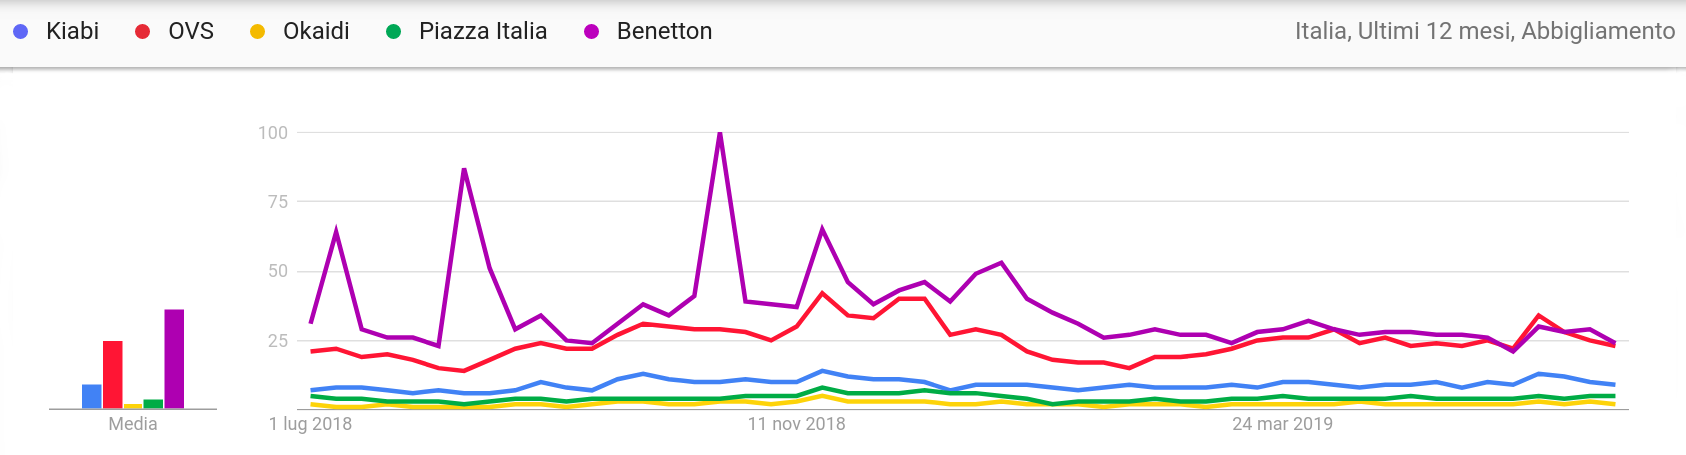
\includegraphics{img/abbigliamento_generico.png}
\caption{Ricerca di mercato - abbigliamento}
\label{abbigliamo_generico}
\end{figure}

Per quanto riguarda il mercato dell'abbigliamento da bambino \cite{gt}, Kiabi perde un ulteriore posizione passando dal terzo al quarto posto, come mostrato in Fig. \ref{abbigliamento_bambino}.

\begin{figure}[h]
\centering
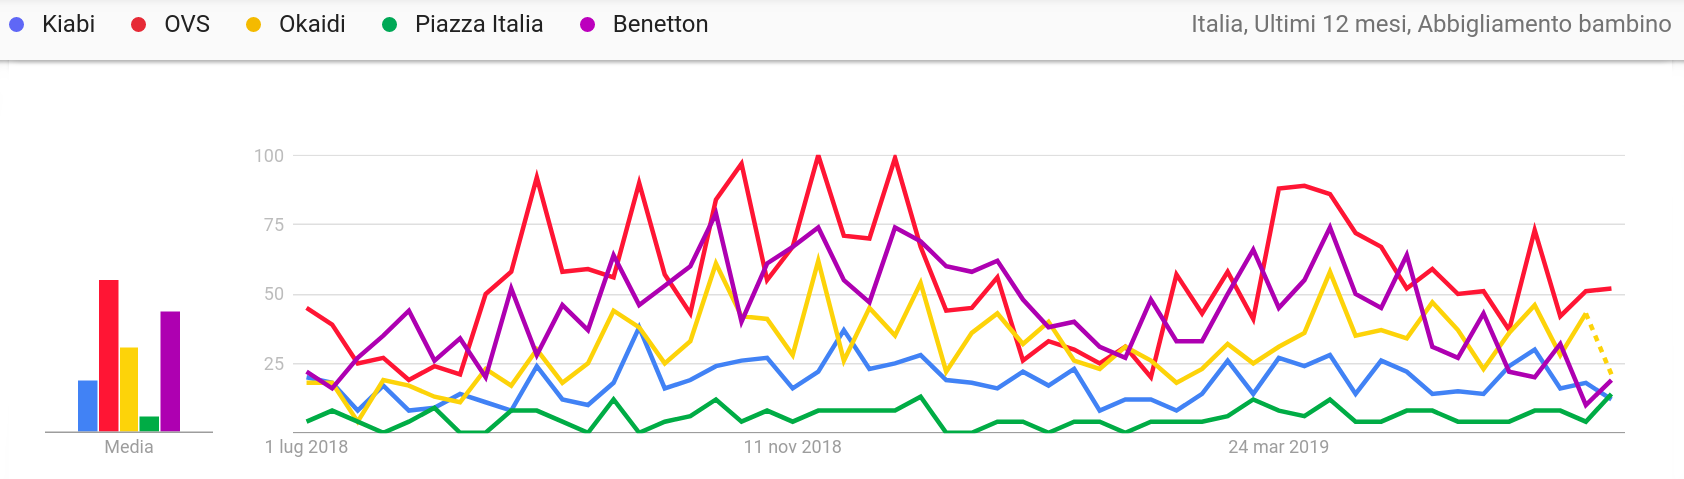
\includegraphics{img/abbigliamento_bambino.png}
\caption{Ricerca di mercato - abbigliamento bambino}
\label{abbigliamento_bambino}
\end{figure}

Dopo un'attenta analisi abbiamo deciso di prendere Kiabi come azienda madre, con l'obiettivo di rilanciarla sul mercato dell'abbigliamento per bambini tramite l'aggiunta di nuove features da noi ideate e proposte al Project Manager Mulliez.

Fare capi estremamente personalizzabili per adulti è più complesso in quanto richiede un investimento iniziale più alto da parte dell'azienda. Al contrario, i capi dedicati ai più piccoli sono suddivisibili per età e non comportano distinzioni tra i sessi. In particolare le magliette per la fascia compresa tra i 3 e i 12 anni risultano essere quelle più facilmente producibili su larga scala offrendo comunque una vasta gamma di personalizzazioni.

\section{Segmentazione utenti}\label{segmentazione_utenti}

La categoria di utenti principali individuata sono:

\begin{itemize}
\item
  \textbf{Persone di età compresa tra i 25 e i 45 anni}

  Kids Experience è stato concepito prendendo come utenti di riferimento
  adulti di entrambi i sessi e di età compresa tra i 25 e i 45 anni. Si
  suppone che gli utenti abbiano una competenza tecnica e di dominio
  media:

  \begin{itemize}
  \tightlist
  \item
    Capacità di utilizzare un browser
  \item
    Capacità di effettuare acquisti su un e-commerce
  \end{itemize}
\item
  \textbf{Stipendio medio}

  Gli utenti di riferimento hanno un reddito annuo di fascia 20k - 30k:
  leggermente più alto rispetto al reddito annuo medio italiano delle
  regioni del centro nord \cite{redditomedio}.
\item
  \textbf{Nazionalità}

  Italiana
\end{itemize}

Si considerano come utenti secondari:

\begin{itemize}
\item
  \textbf{Adulti}

  Tendenzialmente legati agli utenti principali, con compentenze
  tecniche e di dominio nella media:

  \begin{itemize}
  \tightlist
  \item
    Capacità di utilizzare un browser
  \item
    Capacità di effettuare acquisti su un e-commerce
  \end{itemize}
\end{itemize}

\hypertarget{user-research}{%
\section{User research}\label{user-research}}

Per avere un'idea sui comportamenti degli utilizzatori principali del
sito è stata fatta una ricerca tra le varie indagini
di mercato disponibili sul web.
\\
Prendendo in esame l'indagine 
svolta dall'Istituto Nazionale di Statistica (ISTAT) \cite{istat}, si può notare come la spesa media italiana familiare mensile per l'abbigliamento sia di 83.89€.

In particolare ripartita come mostrato in Fig \ref{spesa_media_fam} sulla base del reddito familiare.

\begin{figure}[h]
\centering
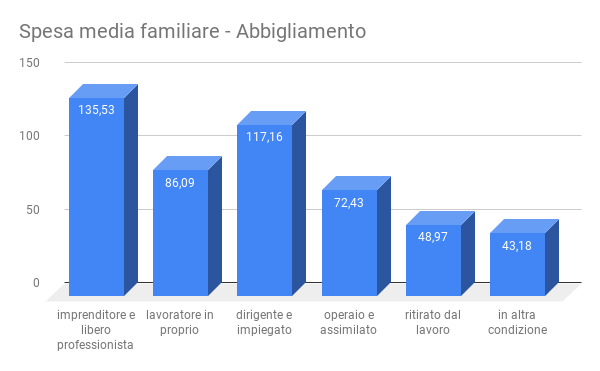
\includegraphics[width=0.75\textwidth]{img/Spesa_media_familiare_abbigliamento.png}
\caption{Spesa media familiare per l'abbigliamento}
\label{spesa_media_fam}
\end{figure}

Dal grafico precedente, estraendo i soli dati riguardanti le famiglie con figli, otteniamo i risultati mostrati in Fig. \ref{spesa_media_n_figli}, dal quale si evince che la spesa più alta è sostenuta dalle famiglie con 2 figli.

\begin{figure}[h]
\centering
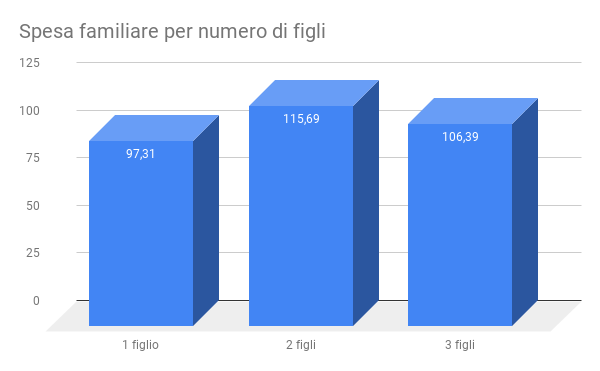
\includegraphics[width=0.75\textwidth]{img/Spesa_familiare_per_numero_di_figli.png}
\caption{Spesa media familiare per numero di figli}
\label{spesa_media_n_figli}
\end{figure}

Per comprendere meglio i bisogni dell'utente target è stata fatta una task analysis, ovvero le operazioni che gli utenti compiono durante il normale utilizzo del sito. Si sono presi in considerazione i principali goal che l'utente dovrebbere raggiungere:
\begin{itemize}
\item creazione di una maglietta personalizzata e salvataggio nei propri progetti personali
\item acquisto di una maglietta
\item condividere un progetto sui social
\end{itemize}

Si suppone che l'utente target acceda al sito tramite desktop.

Elenco task emersi:
\begin{enumerate}
\item Creazione di un account personale su kiabi.it
\item Accesso ai progetti personali
\item Visualizzare i progetti presenti nel catalogo
\item Aggiungere al carrello un prodotto presente nei propri progetti personali
\item Acquisto del contenuto del carrello
\item Creazione di un progetto e condivisione sui social network 
\end{enumerate}

\chapter{Valutazione delle risorse
esistenti}\label{valutazione-delle-risorse-esistenti}

La scelta di prendere Kiabi Italia come sito principale deriva dal fatto che si trova in una posizione sfavorevole rispetto alla concorrenza all'interno del mercato dell'abbigliamento. Pertanto potrebbe essere più interessato e ben propenso alla sperimentazione di novità con l'obiettivo di colmare il gap con la concorrenza.

Come si evince dall'analisi dei dati svolta nel capitolo precedente, le famiglie che spendono di più nel settore dell'abbigliamento sono quelle con stipendi annui sopra la media. Di questi, il picco di spesa lo hanno le famiglie con due figli.

Nella valutazione dei sistemi esistenti, si sono presi in considerazione i due diretti concorrenti di Kiabi:

\begin{itemize}
\tightlist
\item \textbf{OVS}, è una società italiana leader nell'abbigliamento per uomo, donna e bambino. In particolare OVS KIDS si focalizza sui bambini dagli 0 ai 14 anni. In Italia sono presenti 900 negozi fisici.  
\item \textbf{Benetton}, è un'azienda tessile italiana facente parte del marchio United Colors of Benetton. I suoi prodotti spaziano dall'abbigliamento, agli accessori e alle calzature. In italia sono presenti 944 negozi fisici.
\end{itemize}

Kiabi è stato preferito agli altri due competitor per i motivi sopracitati. Inoltre Kiabi, non possedendo tanti negozi fisici quanti quelli dei suoi concorrenti, cerca di vendere il più possibile tramite lo store online. Infatti possiede intere linee di prodotti dedicati esclusivamente alla vendita online.

\section{Expert Usability Review}\label{expert-usability-review}

L'expert usability review prevede che un esperto di usabilità ispezioni il sito per identificare potenziali problemi.

A differenza dello usability testing questo non coinvolge gli utenti.

Nonostante sia meno potente, l'expert usability review permette di trovare i problemi più grossolani in modo semplice e veloce.

L'analisi effettuata in questa fase è avvenuta adottando come linee guida
``le 10 euristiche di Nielsen e Molich'' e a tali euristiche sono state
affiancate alcune delle euristiche di Weinshenk e Barker:

\begin{enumerate}
\def\labelenumi{\arabic{enumi}.}
\item
  \textbf{Visibilità dello stato del sistema}

  Il sistema dovrebbe tenere sempre l'utente informato su cosa succede
  nel sistema attraverso l'uso di feedback appropriati forniti in tempi
  ragionevoli.
\item
  \textbf{Corrispondenza tra sistema e mondo reale}

  Il sistema dovrebbe ``parlare'' la lingua dell'utente con parole,
  frasi e concetti familiari all'utente invece che utilizzare termini
  propri del sistema.
\item
  \textbf{Controllo e libertà}
  Dato che l'utente spesso usa delle funzionalità del sistema per
  errore, è sempre necessario fornire un modo per uscire dallo stato in
  cui si è venuto a trovare.
\item
  \textbf{Consistenza e standard}
  L'utente non dovrebbe avere dubbi riguardo al fatto che parole,
  situazioni, azioni differenti abbiano lo stesso effetto.
\item
  \textbf{Prevenzione dell'errore}

  Il miglior modo per evitare un errore è prevenirlo.
\item
  \textbf{Riconoscimento anziché ricordo}

  Minimizzare il carico cognitivo dell'utente rendendo gli oggetti, le
  azioni e le opzioni più visibili possibili. Gli utenti non dovrebbero
  ricordare le informazioni da un dialogo all'altro.
\item
  \textbf{Flessibilità ed efficienza d'uso}

  Il sistema deve facilitare l'uso anche agli utenti esperti,
  permettendogli di personalizzare le azioni più frequenti.
\item
  \textbf{Design ed estetica minimalista}

  I dialoghi non dovrebbero contenere informazioni che sono irrelevanti
  o di cui si ha raramente bisogno. Ogni informazione extra compete con
  le informazioni rilevanti e diminuisce la loro visibilità.
\item
  \textbf{Aiuto all'utente}

  Gli errori dovrebbero essere mostrati in un linguaggio chiaro,
  indicando in modo preciso il problema e suggerendo la soluzione.
\item
  \textbf{Documentazione}


Sarebbe meglio fornire un'adeguata documentazione, a presciendere dal
fatto che il sito potrebbe essere utilizzato anche senza. Questo genere
di informazione dovrebbe essere facile da cercare, focalizzata sul task
dell'utente e dovrebbe elencare una sequenza di passi semplici da
completare.

\def\labelenumi{\arabic{enumi}.}
\setcounter{enumi}{10}
\item
    \textbf{Predicibilità}

L'utente sarà in grado di costruire un modello mentale di come il
sistema risponderà alle sue azioni.

\def\labelenumi{\arabic{enumi}.}
\setcounter{enumi}{11}
\item
  \textbf{Limitazioni umane}

Il design deve tener conto delle limitazioni cognitive e sensoriali per
evitare un sovraccarico cognitivo.

\def\labelenumi{\arabic{enumi}.}
\setcounter{enumi}{12}
\item
  \textbf{Precisione}

L'interfaccia permette all'utente di portare a termine il task con
esattezza
\end{enumerate}


\subsubsection{Prima Ispezione - Kiabi}\label{prima-ispezione}
Si procede ora con una prima fase di ispezione del sistema esistente (kiabi.it) analizzando nel complesso il tipo di servizio che offre all’utente, a chi si rivolge principalmente il sistema, ed eventuali problemi riscontrati durante la navigazione.

Il sito presenta una schermata iniziale pulita. Al centro della pagine figura un banner che mostra le offerte del momento. Questo è inoltre corredato di collegamenti alle sezioni principali. 

Con uno scroll verso il basso si accede ad una serie di carusel che mostrano gli articoli disponibili suddivisi per filtri (es. ultimi arrivati, in offerta, ecc).
In ogni pagina sono inoltre presenti delle breadcrumb che mostrano la posizione dell'utente all'interno del sito.

La struttura è uguale in tutte le pagine ed è formata da navbar, footer (uguali per ogni pagina) e la sezione centrale con il contenuto della pagina interessata.

La navbar contiene i link alle principali categorie di prodotti esposte nel sito:

\begin{itemize}
\item Novità
\item Donna
\item Intimo
\item Uomo
\item Taglie forti
\item Bambino/a
\item Scarpe
\end{itemize}

Il footer contiene una serie di link di utilità:

\begin{itemize}
\item Aiuto
\item Servizi
\item Informazioni
\item Follow us
\end{itemize}

Da notare che viene prestata particolare attenzione alla facilitazione degli utenti inesperti o affetti da deficit fisici. Sotto la sezione aiuto oltre alla classica F.A.Q. sono presenti videotutorial sottotitolati per utenti non udenti e la sezione "Contattaci" dove è possibile contattare direttamente l'assistenza sia telefonicamente che in chat.

Per poter procedere ad un acquisto l'utente deve selezionare dalla navbar la categoria di interesse.
A questo punto viene mostrato l'intero catalogo relativo alla categoria selezionata con la possibilità di applicare filtri quali: prezzo, colore, categorie.

Una volta selezionato un prodotto si viene indirizzati alla pagina contenente i dettagli. Questa è suddivisa in due sezioni, una destra e una sinistra.
La parte destra oltre a contenere le immagini del prodotto, espone anche una breve descrizione di questo. 
Nella parte sinistra sono mostrate le informaizoni riguardati il prezzo ed eventuali saldi, nonchè viene offerta la possiblità di selezionare taglia e colore. La stessa sezione permette anche di aggiungere l'articolo al carrello.

Una volta nel carrello per completare l'acquisto sono sufficienti pochi click. Dopo aver clickkato su completa ordine viene richiesto il metodo di pagamento e in uno step successivo anche l'indirizzo di spedizione. Si giunge infine alla schermata di riepilogo con il totale.


Dalle ricerche effettuate il target di utenza di kiabi è composto principalmente da:
\begin{itemize}
    \item Utenti Francesi, Spagnoli, Italiani
    \item Età compresa tra 16 e 50 anni
    \item Reddito medio basso
\end{itemize}

Il 26 novembre 2014 kiabi crea ad Angers il primo negozio a marchio Kiabi Kids, dedicato esclusivamente all'abbigliamento per i bambini 0-16 anni. L'azienda dimostra di essere fortemente interessata al mercato dell'abbigliamento dedidcato ai più piccoli.



\subsubsection{Analisi diretta: Sistema - Linee
guida}\label{analisi-diretta-sistema---linee-guida}


Non sono state riscontrate particolari criticità durante la navigazione. L'interfaccia risulta essere snella ed intuitiva. Volendo trovare forzatamente un difetto, questo potrebbe essere individuato nella schermata di login. Questa si presenta all'utente prima con la label "login" e successivamente con "connettiti". Il sistema non parla lo stesso linguaggio dell'utente. Non rispetta l'euristica della \emph{Corrispondenza tra sistema e mondo reale}.



\hypertarget{analisi-inversa-linee-guida---sistema}{%
\subsubsection{Analisi inversa: Linee guida -
Sistema}\label{analisi-inversa-linee-guida---sistema}}

Con l'analisi inversa vengono confrontate le linee guida con il sistema, utilizzando le euristiche sopradescritte e mettendo in evidenza quelle che non vengono rispettate.
\begin{enumerate}
\def\labelenumi{\arabic{enumi}.}
\tightlist
\item
  \textbf{Visibilità dello stato del sistema}: euristica pienamente rispettata grazie alle breadcrumb presenti in ogni pagina/sezione.
\item
  \textbf{Corrispondenza tra sistema e mondo reale}: eccezion fatta per la problematica descritta nell'analisi diretta, non sono state riscontrate violazioni.
\item
  \textbf{Controllo e libertà}: una volta selezionato un prodotto è possibile ritornare al catalogo utilizzando le breadcrumb. Tuttavia questo presenta una problematica, scrollando le pagine queste vengono nascoste dalla navbar.
\item
  \textbf{Consistenza e standard}: l'interfaccia presenta elementi come footer e navbar che la rendono consistente. La filosofia minimale largamente applicata nel sito si attiene agli standard.
\item
  \textbf{Prevenzione dell'errore}: in ogni momento l'utente è conscio dello stato di avanzamento delle operazioni che sta eseguendo. 
\item
  \textbf{Riconoscimento anziché ricordo}: l'interfaccia raccoglie in ogni momento le informazioni essenziali. L'unica nota negativa emerge navigando il catalogo. Per ogni oggetto l'utente può visionare la disponibilità di un prodotto (taglia/colore) solo facendo hover sul prodotto stesso.
\item
  \textbf{Flessibilità d'uso}: per natura del sistema non è necessario fornire short cut dedicate all'utente esperto. Tutte le azioni possibili sono eseguibili in pochi passi e con estrema semplicità. Unica personalizzazione possibile e di grande efficacia è la possibilità di decidere il numero di elementi visualizzabili in una pagina consentendo all'utente esperto di poter accedere a più prodotti senza dover cambiare pagina.
\item
  \textbf{Design ed estetica minimalista}: il catalogo è esposto magistralmente. Ci sono solo tre elementi per riga che mostrano l'unica cosa importante per l'utente: l'immagine del prodotto. Inoltre le opzioni di default permettono di arrivare in fondo con pochi scroll. 
\item
  \textbf{Aiuto all'utente}: il sistema è progettato per rendere le possibilità di errori infinitesimali. L'unica operazione potenzialmente "irreversibile", ossia l'acquisto, richiede l'attraversamento di ben tre step con relativa conferma da parte dell'utente. 
  E' sempre possibile tornare indietro in ogni step. Anche dopo la fase di pagamento è possibile annullare l'ordine sino a prima della partenza. In tal caso l'utente può effettuare la restituzione.
\item
  \textbf{Documentazione}: inesistente
\item
  \textbf{Predicibilità}: euristica rispettata
\item
  \textbf{Limitazioni umane}: euristica rispettata
\item
  \textbf{Precisione}: euristica rispettata
\end{enumerate}

\section{User testing}\label{user-testing}

In seguito alla mancanza di un team specializzato per il testing del
software si è deciso di usare il \emph{discount usability testing}
proposta da Nielsen, nello specifico la metodologia di testing usata è
\emph{Thinking Aloud}.

Sono stati dunque scelti 4 utenti che rispettano il target scelto e ad
ognuno di loro è stato chiesto di portare a termine 4 task per poter
osservare gli errori e i punti critici del sistema.

\subsection{Protocollo di testing}\label{protocollo-di-testing}

\begin{itemize}
\item
  \textbf{Tipologia}: Discount usability testing
\item
  \textbf{Metodologia}: Thinking Aloud
\item
  \textbf{Task da testare}: 
  
  \begin{enumerate}
  \def\labelenumi{\arabic{enumi}.}
  \tightlist
  \item
    Acquistare un prodotto
  \item
    Cercare, tramite la barra di ricerca, dei pantaloni da uomo di colore blu, taglia L
  \item
    Inserire un prodotto nella whishlist
  \item
    Visualizzare un prodotto da bambini nella sezione "Esclusivo per il web"
  \end{enumerate}
\item
  \textbf{Descrizione dei risultati}:

  \begin{itemize}
  \item
    \textbf{Sfumature sul compimento del task}: necessità di
    suggerimenti da parte degli osservatori
  \item
    \textbf{Errori}:

    \begin{itemize}
   
    \item
      Catastrofici: fallimento del task
    \item
      Gravi: rallentamento notevole nell'esecuzione del task
    \item
      Minori: rallentamento sensibile nell'esecuzione del task
    \item
      Cosmetici: fastidio all'utente senza rallentamento visibile
      nell'esecuzione del task
    \end{itemize}
  \end{itemize}
\item
  \textbf{Domande post-sessione}:

  \begin{itemize}
  \tightlist
  \item
    System Usability Scale (SUS)
  \end{itemize}
\item
  \textbf{Scelta dei soggetti}: effettuata di comune accordo con i
  membri del team
\item
  \textbf{Organizzazione del test}: test condotti in presenza del team
\end{itemize}

\hypertarget{risultati-test}{%
\subsection{Risultati test}\label{risultati-test}}

Ad ogni utente sono stati proposti i quattro task sopracitati da realizzare sul sito, ovvero quattro compiti specifici da portare a termine utilizzando l'interfaccia dal sito Kiabi. 

I task sono stati scritti su carta e presentati all'utente.
L'osservatore si è preoccupato di preparare l'ambiente per lo
svolgimento del test e di spiegare al tester il motivo del testing,
mettendolo a suo agio spiegando che è il sistema ad essere valutato e
non le sue capacità e, in caso cui fosse stato troppo in silenzio o
bloccato su un punto, ha cercato di spingerlo a provare nuovamente senza
fornire alcun aiuto esplicito. Durante il testing l'osservatore ha preso
appunti segnando eventuali problemi incontrati.

Alla fine del test è stato proposto all'utente il questionario SUS così
formato:

\begin{enumerate}
\def\labelenumi{\arabic{enumi}.}
\tightlist
\item
  Penso che userei questo sistema con frequenza
\item
  Ho trovato il sistema troppo complesso
\item
  Penso che il sistema sia facile da usare
\item
  Penso che avrei bisogno dell'aiuto di una persona esperta per essere
  in grado di usare il sistema
\item
  Ritengo che le varie funzionalità di questo sistema siano ben
  integrate
\item
  Ritengo che il sistema sia inconsistente
\item
  Penso che la maggior parte della gente sia in grado di imparare
  velocemente ad usare questo sistema
\item
  Ritengo che il sistema sia poco maneggevole
\item
  Mi sono sentito molto sicuro nell'utilizzo del sistema
\item
  Ho avuto bisogno di imparare molte cose prima di sentirmi sicuro nell'utilizzo del sistema
\end{enumerate}

Sono stati selezionati 4 soggetti rientranti nel target di Kiabi per lo svolgimento dei test: 
\begin{itemize}
\item Donna, 35 anni, interesse nella moda e conoscenza basilare del computer;
\item Uomo, 25 anni, scarsa conoscenza delle ultime tendenze e buona conoscenza tecnica del computer, in particolare e-commerce;
\item Donna, 22 anni, iscritta alla facoltà di "Culture e pratiche della moda". Buona conoscenza del computer;
\item Uomo, 38 anni, completo disinteresse per la moda, ma con spiccato senso pratico. Scarsa conoscenza del computer.
\end{itemize} 

Sono state scelte le seguenti metriche per la valutazione dell'usabilità del sistema:

\begin{itemize}
\item
  Svolgimento: successo, fallimento
\item
  Errori: Nielsen
\item
  Efficienza: alta, media, bassa
\end{itemize}

\subsubsection{Raccolta dati}\label{raccolta-dati}

\begin{longtable}[]{@{}lllll@{}}
\toprule
Giorgio & Task 1 & Task 2 & Task 3 & Task 4\tabularnewline
\midrule
\endhead
Svolgimento & Successo & Successo & Successo & Fallimento\tabularnewline
Errori & / & Errore cosmetico & Errore Minore & Errore
grave\tabularnewline
Efficienza & Alta & Alta & Media & Bassa\tabularnewline
\bottomrule
\end{longtable}

Risposte questionario SUS:

\begin{longtable}[]{@{}ll@{}}
\toprule
Domanda & Risposta\tabularnewline
\midrule
\endhead
1 & 2\tabularnewline
2 & 1\tabularnewline
3 & 4\tabularnewline
4 & 1\tabularnewline
5 & 2\tabularnewline
6 & 4\tabularnewline
7 & 2\tabularnewline
8 & 3\tabularnewline
9 & 5\tabularnewline
10 & 2\tabularnewline
\bottomrule
\end{longtable}

\begin{longtable}[]{@{}lllll@{}}
\toprule
Francesco & Task 1 & Task 2 & Task 3 & Task 4\tabularnewline
\midrule
\endhead
Svolgimento & Successo & Successo & Successo & Successo\tabularnewline
Errori & / & Errore cosmetico & Errore Minore & Errore cosmetico
grave\tabularnewline
Efficienza & Alta & Media & Bassa & Media\tabularnewline
\bottomrule
\end{longtable}

Risposte questionario SUS:

\begin{longtable}[]{@{}ll@{}}
\toprule
Domanda & Risposta\tabularnewline
\midrule
\endhead
1 & 3\tabularnewline
2 & 2\tabularnewline
3 & 3\tabularnewline
4 & 1\tabularnewline
5 & 4\tabularnewline
6 & 3\tabularnewline
7 & 2\tabularnewline
8 & 2\tabularnewline
9 & 4\tabularnewline
10 & 1\tabularnewline
\bottomrule
\end{longtable}

\begin{longtable}[]{@{}lllll@{}}
\toprule
Sofia & Task 1 & Task 2 & Task 3 & Task 4\tabularnewline
\midrule
\endhead
Svolgimento & Successo & Successo & Successo & Fallimento\tabularnewline
Errori & / & / & Errore minore & Errore catastrofico
grave\tabularnewline
Efficienza & Alta & Alta & Media & Bassa\tabularnewline
\bottomrule
\end{longtable}

Risposte questionario SUS:

\begin{longtable}[]{@{}ll@{}}
\toprule
Domanda & Risposta\tabularnewline
\midrule
\endhead
1 & 3\tabularnewline
2 & 2\tabularnewline
3 & 4\tabularnewline
4 & 1\tabularnewline
5 & 2\tabularnewline
6 & 4\tabularnewline
7 & 4\tabularnewline
8 & 4\tabularnewline
9 & 4\tabularnewline
10 & 2\tabularnewline
\bottomrule
\end{longtable}

\begin{longtable}[]{@{}lllll@{}}
\toprule
Eva & Task 1 & Task 2 & Task 3 & Task 4\tabularnewline
\midrule
\endhead
Svolgimento & Successo & Fallimento & Successo & Fallimento\tabularnewline
Errori & / & Errore catastrofico & / & Errore grave
grave\tabularnewline
Efficienza & Alta & Bassa & Media & Bassa\tabularnewline
\bottomrule
\end{longtable}

Risposte questionario SUS:

\begin{longtable}[]{@{}ll@{}}
\toprule
Domanda & Risposta\tabularnewline
\midrule
\endhead
1 & 4\tabularnewline
2 & 3\tabularnewline
3 & 2\tabularnewline
4 & 2\tabularnewline
5 & 3\tabularnewline
6 & 3\tabularnewline
7 & 4\tabularnewline
8 & 3\tabularnewline
9 & 4\tabularnewline
10 & 1\tabularnewline
\bottomrule
\end{longtable}

\subsubsection{Punteggi questionario SUS}\label{punteggi-SUS}

Al termine di ogni test è stato proposto ad ogni utente un questionario di soddisfazione composto da dieci affermazioni. Le risposte sono state date utilizzando la \emph{Scala di Likert} con valori compresi tra 1 e 5, dove 1 significa essere completamente in disaccordo con l'affermazione data, mentre 5 essere completamente d'accordo.

\begin{longtable}[]{@{}lllllllllllll@{}}
\caption{Riepilogo risposte SUS}\tabularnewline
\toprule
& 1 & 2 & 3 & 4 & 5 & 6 & 7 & 8 & 9 & 10 & Somma & Totale\tabularnewline
\midrule
\endfirsthead
\toprule
& 1 & 2 & 3 & 4 & 5 & 6 & 7 & 8 & 9 & 10 & Somma & Totale\tabularnewline
\midrule
\endhead
Giorgio & 2 & 1 & 4 & 1 & 2 & 4 & 2 & 3 & 5 & 2 & 24 & 60\tabularnewline
Francesco & 3 & 2 & 3 & 1 & 4 & 3 & 2 & 2 & 4 & 1 & 27 &
67,5\tabularnewline
Sofia & 3 & 2 & 4 & 1 & 2 & 4 & 4 & 4 & 4 & 2 & 24 &
60\tabularnewline
Eva & 4 & 3 & 2 & 2 & 3 & 3 & 4 & 3 & 4 & 1 & 25 &
62,5\tabularnewline
\bottomrule
\end{longtable}

Visti i risultati ottenuti nei questionari SUS possiamo affermare che Kiabi ha sia una \emph{Learnability}, ovvero la capacità di apprendimento, che una \emph{Usability} nella media.

Di seguito i problemi riscontrati durante i test:

\begin{itemize}
\item Il pulsante a forma di cuore, che dovrebbe inserire un prodotto nella whishlist, funziona solamente dopo essere entrati nel dettaglio prodotto (\textbf{E1})
\item Le taglie dei prodotti alcune volte sono specificate con lo standard italiano, mentre altre volte con quello americano o francese (\textbf{E2})
\item Le breadcrumb presenti in tutte le sottosezioni del sito, risultano essere di scarsa visibilità a causa del font e delle dimensioni (\textbf{E3})
\end{itemize}

\begin{longtable}[]{@{}llllll@{}}
\toprule
Errore & Implementativo & Catastrofico & Grave & Minore &
Cosmetico\tabularnewline
\midrule
\endhead
E1 & X & & X &\tabularnewline
E2 & & & & & X\tabularnewline
E3 & & & X & &\tabularnewline
\bottomrule
\end{longtable}

\subsubsection{Curva d'urgenza}

La curva d'urgenza è un grafico bidimensionale ``impatto vs frequenza'' in cui sono presenti i vari errori riscontrati.

\begin{figure}[h]
\caption{Curva d'urgenza di Kiabi}
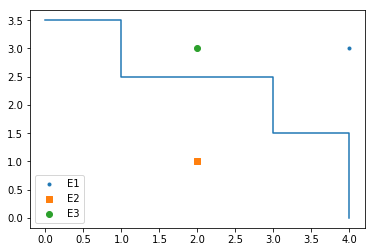
\includegraphics[width=0.90\textwidth]{img/curve_urgenza_kiabi}
\centering
\end{figure}

Durante i test sono stati riscontrati, fondamentalmente, tre problematiche.

La prima problematica riguarda la scarsa usabilità della whishlist. Gli utenti si aspettavano, nel loro modello mentale, che una volta premuto il bottone a forma di cuore il prodotto fosse inserito immediatamente nella whishlist. Dopo un'attenta analisi si è notato che tale funzionalità è disponibile solamente dopo aver selezionato la taglia che compare tramite menù drop-down nell'anteprima del prodotto, non sempre visibile. Tuttavia non c'è nulla che indichi la corretta sequenza di azioni all'utente.

Per quanto riguarda la seconda problematica, c'è una inconsistenza nel modo in cui vengono esposte le taglie dei vari prodotti.

Infine le breadcrumb non sembrano essere la scelta giusta come metodo di navigazione del sito. Durante lo scroll della pagina, queste scompaiono. Anche quando visibili, non sempre l'utente le riesce ad individuare a causa delle ridotte dimensioni.

\chapter{Studio di fattibilità}\label{studio-di-fattibilituxe0}

In questa fase verranno analizzati i ``Contesti d'uso'', gli
``Scenarios'' e le ``Personas''.

I ``Contesti d'uso'' descrivono in modo chiaro e preciso le
caratteristiche degli utenti target, i task che dovranno svolgere e
gli eventuali vincoli presenti.

Gli ``Scenarios'' sono brevi storie che raccontano in dettaglio come
l'utente realizza l'obiettivo personale eseguendo uno o più dei compiti
pianificati sul sistema.

Infine si rappresenteranno le ``Personas'', ovvero verranno descritti,
in modo dettagliato, gli utenti che utilizzeranno il sistema.

\hypertarget{contesto-duso}{%
\section{Contesto d'uso}\label{contesto-duso}}

Gli utenti che utilizzeranno il sistema si suppone siano persone con uno spiccato senso di creatività e un minimo di interesse per la moda. Si presume abbiano un reddito leggermente sopra la media nazionale, in modo da potersi permettere un prodotto, che probabilmente sarà un regalo, che è piuttosto ricercato e non semplicemente acquistabile nei negozi fisici, come appunto una maglietta personalizzata.

Una buona parte degli utenti, sia maschile che femminile, avrà un/una figlio/a (3 - 12 anni). 
Più in generale, l'utente target sarà colui che per via di amici, parenti o colleghi, si trova nella situazione di dover fare un regalo ad un bambino/a.

Le attività che l'utente potrà svolgere sul sito saranno:
\begin{itemize}
\item Creazione di una maglietta personalizzata, nello specifico: 
\begin{itemize}
\item scegliere fra un'ampia gamma di personalizzazioni per ogni singola parte della maglietta
\end{itemize}
\item Visualizzazione delle magliette salvate
\item Visualizzazione delle magliette create dagli altri utenti
\item Condivisione sui social di una maglietta creata
\item Acquisto di una maglietta
\end{itemize}

\subsection{Vincoli ambientali}\label{vincoli-ambientali}

Si presuppone un utilizzo tipico del sito per gli acquisti in un ambiente tranquillo come quello domestico o simili, dove l'utente si possa concentrare, se necessario, nella personalizzazione dei prodotti.
Tale ambiente non comporta quindi vincoli particolari.

\subsection{Vincoli tecnici}\label{vincoli-tecnici}

Il sito web richiede una connessione ad Internet per essere utilizzato.
L'interfaccia è progettata, con le tecnologie attuali, in maniera tale da garantire e supportare una buona esperienza di utilizzo da PC.
Inoltre a causa delle potenzialità di personalizzazione dell'editor, risulta obbligatorio l'accesso da dispositivi notebook o desktop.

\subsection{Vincoli culturali}\label{vincoli-culturali}

Non ci sono particolari vincoli culturali in quanto il servizio è pensato solamente per utenti italiani, presentando tutti i testi in lingua italiana. 

\section{Scenarios}\label{scenarios}

\hypertarget{severina-millanta---qualcosa-di-unico-per-la-bambina}{%
\subsection{Severina Millanta - Qualcosa di unico per la
bambina}\label{severina-millanta---qualcosa-di-unico-per-la-bambina}}

Sta per arrivare il compleanno della bambina e Severina ha già
provveduto a organizzare una festa in cui invitare i compagni di scuola
e relativi genitori.

Dopo aver organizzato la festa non resta che pensare al regalo. Parlando
con le altre mamme ha convenuto che la cosa migliore sarebbe comprare un
capo di abbigliamento. Severina però non vuole ripiegare sulle classiche
cose che si possono reperire nei negozi, vuole qualcosa di unico che
parli della sua bambina e che le faccia fare bella figura con le altre
mamme. Inizialmente pensa di recarsi da un sarto, ma dato il costo e il
tempo di attesa capisce subito che non è la scelta vincente.

Inizia a scrivere post spiegando la problematica su un paio di forum.
Tra i vari consigli ne spunta uno che risponde esattamente alle sue
esigenze: facile da usare, altamente personalizzabile e veloce nella
consegna.

\hypertarget{antonio-frastani---una-maglietta-da-campione}{%
\subsection{Antonio Frastani - Una maglietta da
campione}\label{antonio-frastani---una-maglietta-da-campione}}

Da alcuni giorni la sua ragazza non fa altro che raccontare ad Antonio
le avventure del suo primo nipotino. Il bambino, a quanto pare, passa le
giornate al parco a giocare a calcio con gli amici e sogna da grande di
entrare in una squadra professionistica.

Antonio, dopo una lunga giornata di lavoro, decide di fare un regalo al
nipote della sua ragazza. Antonio si mette a cercare su Google un
possibile regalo per un bambino di 7 anni. Su un forum di settore gli
viene consigliata la possibilità di creare una maglia personalizzata
basandosi su quella della propria squadra del cuore.

Subito Antonio si fionda su Kids Experience per osservare il catalogo e
le personalizzazioni disponibili. Non essendo una persona creativa si
accontenta di uno dei modelli più votati e in pochi minuti procede con
l'ordine.

\hypertarget{diego-de-la-vega---la-maglia-della-salute}{%
\subsection{Diego de la Vega - La maglia della
salute}\label{diego-de-la-vega---la-maglia-della-salute}}

Tra pochi giorni, all'interno della palestra in cui lavora Diego, si
terrà l'inaugurazione di un nuovo corso di ginnastica artistica per i
bambini delle scuole elementari. Il responsabile di questo corso ha
chiesto a tutti i personal trainer di ideare delle magliette carine, che
possano essere utilizzate durante le lezioni, da distribuire a tutti i
bambini come regalo di benvenuto durante l'inaugurazione.

Chiedendo a i suoi colleghi viene a conoscenza di Kids Experience. Una
volta a casa, dopo essersi preso del tempo per riposare, Diego accende
il suo computer portatile, accede al sito Kids Experience e inizia a
creare delle magliette sia per i bambini che per le bambine del nuovo
corso di ginnastica artistica. Una volta ultimati i prototipi li mostra
alla sorella Sofia e alla mamma Adriana per chiedere i loro pareri.
Successivamente li invia tramite mail al responsabile del corso e li
condivide sui social per sentire anche il parere di amici e conoscenti.

Nonostante la poca fantasia di Diego, grazie al sito Kids Experience che
offre un'ampia gamma di personalizzazioni, facili e intuitive da
utilizzare, si può ritiene soddisfatto delle sue creazioni.

\hypertarget{elisa-pezzana---colazione-da-tiffany}{%
\subsection{Elisa Pezzana - Colazione da
Tiffany}\label{elisa-pezzana---colazione-da-tiffany}}

Si avvicina il giorno di compleanno della figlia ed Elisa non sa cosa
regalarle, così una domenica mattina al bar con le amiche chiede loro
alcuni consigli su qualcosa di originale e adatto ad una bambina di 13
anni. Una sua amica le consiglia di regalarle una maglietta
personalizzata da creare online sul sito web Kids Experience, in quanto
è semplice da usare ed è molto veloce nella consegna.

Tornata a casa, approfittando dell'assenza della figlia, accende il computer per accedere al sito che le è stato consigliato per creare una maglietta personalizzata. Pur non avendo molte competenze tecnologiche riesce a personalizzare una maglietta grazie all'interfaccia snella e intuitiva
offerta dalla piattaforma e guardando ciò che gli altri utenti hanno personalizzato.

\hypertarget{giorgia-moro---tutto-bene-quel-che-finisce-bene}{%
\subsection{Giorgia Moro - Tutto è bene quel che finisce
bene}\label{giorgia-moro---tutto-bene-quel-che-finisce-bene}}

Dopo un'intensa giornata lavorativa, Giorgia, una volta tornata a casa,
approfittando dell'assenza di Alice che si trova a giocare al parco
insieme ad alcune amiche, sotto la supervisione di Andrea, decide di
iniziare a cercare online un regalo per l'imminente compleanno della
figlia. Quest'anno Giorgia vorrebbe regalare ad Alice una maglietta che
segua le ultime tendenze in fatto di moda e che possa sfoggiare durante
la prossima vacanza estiva a Tenerife, senza, però, spendere un
capitale.

A questo punto Giorgia prende il suo portatile, lo accende e inizia a
sfogliare i cataloghi online di importanti marchi di moda come Gucci,
Louis Vuitton e Prada per cercare qualche ispirazione e vedere le loro
ultime creazioni. Inoltre, leggendo ormai da anni Vanity Fair, Giorgia
ha acquisito una buona conoscenza in fatto di moda.

Dopo essersi informata sui social, accede a Kids Experience e nonostante
la sua inesperienza con il computer, grazie alla semplicità di utilizzo
della piattaforma, riesce in breve tempo a creare la maglietta perfetta
per il compleanno di Alice. Molto soddisfatta della sua creazione,
Giorgia non vede l'ora che la maglietta le venga recapitata a casa.
\newpage
\hypertarget{personas}{%
\section{Personas}\label{personas}}

Il cast è diviso in:

\begin{itemize}
\tightlist
\item
  protagonista, ossia la personas i cui bisogni devono essere soddisfatti
  al 100\%
\item
  personaggi secondari, che riguardano storie di contorno
\end{itemize}

\hypertarget{protagonista}{%
\subsection{Protagonista}\label{protagonista}}

\hypertarget{severina-millanta}{%
\subsubsection{Severina Millanta}\label{severina-millanta}}

\begin{figure}[h]
\centering
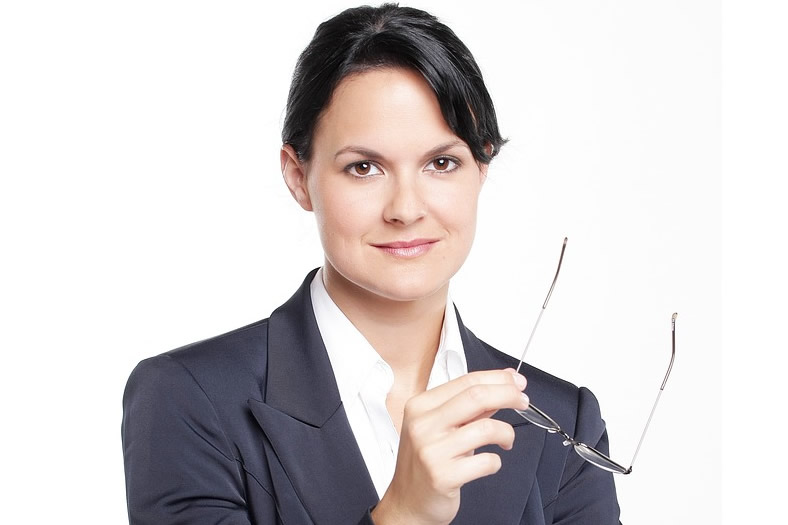
\includegraphics[width=0.50\textwidth]{img/severina.jpg}
\end{figure}

\begin{longtable}[h]{@{}ll@{}}
\toprule
& Severina Millanta\tabularnewline
\midrule
\endhead
Età & 42\tabularnewline
Sesso & F\tabularnewline
Impiego & Ragioniera\tabularnewline
Figli & Una figlia di 10 anni\tabularnewline
Hobby & Cucina, nuoto\tabularnewline
Uso di internet & 80\% casa, 5\% lavoro, 15\% altrove\tabularnewline
\bottomrule
\end{longtable}

\newpage
\hypertarget{personaggi-secondari}{%
\subsection{Personaggi secondari}\label{personaggi-secondari}}

\hypertarget{antonio-frastani}{%
\subsubsection{Antonio Frastani}\label{antonio-frastani}}

\begin{figure}[h]
\centering
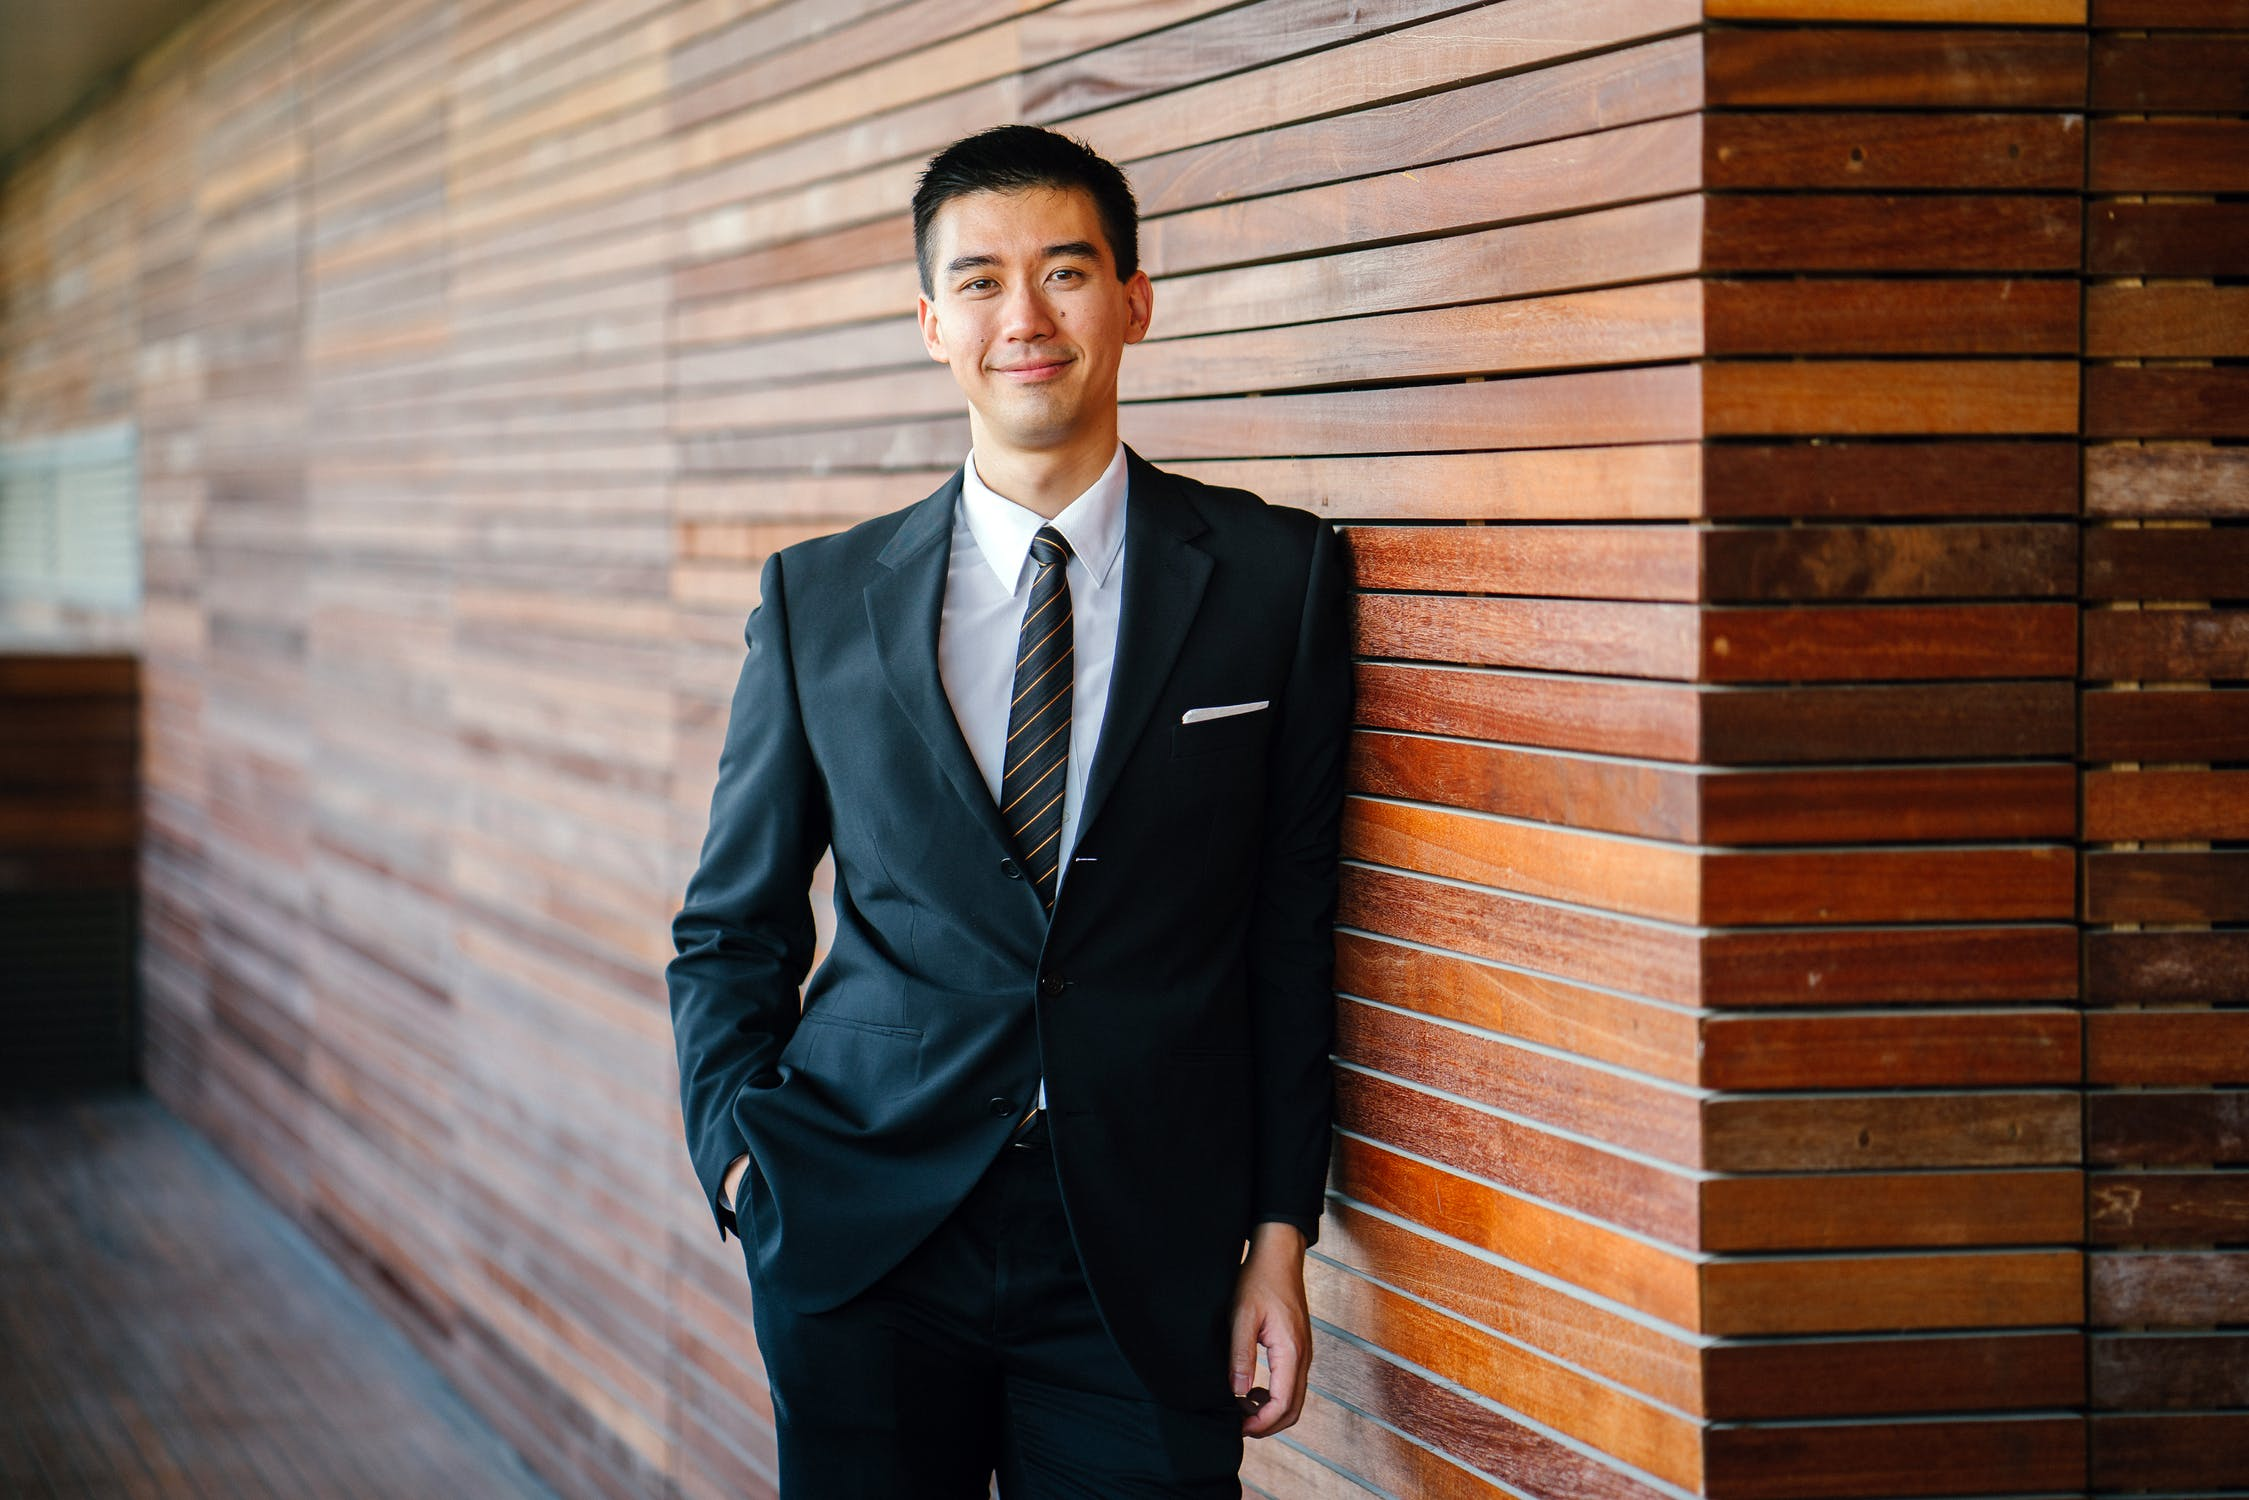
\includegraphics[width=0.5\textwidth,height=\textheight]{img/antonio.jpeg}
\end{figure}

\begin{longtable}[]{@{}ll@{}}
\toprule
& Antonio Frastani\tabularnewline
\midrule
\endhead
Sesso & M\tabularnewline
Impiego & Impiegato bancario\tabularnewline
Figli & No\tabularnewline
Hobby & Motori\tabularnewline
Uso di internet & 70\% casa 20\% ufficio 10\% altro\tabularnewline
\bottomrule
\end{longtable}


\newpage
\hypertarget{diego-de-la-vega}{%
\subsubsection{Diego de la Vega}\label{diego-de-la-vega}}

\begin{figure}[h]
\centering

\includegraphics[width=0.5\textwidth,height=\textheight]{img/diego.jpg}
\end{figure}

\begin{longtable}[]{@{}ll@{}}
\toprule
& Diego de la Vega\tabularnewline
\midrule
\endhead
Sesso & M\tabularnewline
Impiego & Personal Trainer\tabularnewline
Figli & No\tabularnewline
Hobby & Sport\tabularnewline
Uso di internet & 60\% lavoro 30\% casa 10\% altro\tabularnewline
\bottomrule
\end{longtable}

\hypertarget{elisa-pezzana}{%
\subsubsection{Elisa Pezzana}\label{elisa-pezzana}}

\begin{figure}[h]
\centering

\includegraphics[width=0.5\textwidth,height=\textheight]{img/elisa.jpg}
\caption{Elisa Pezzana}
\end{figure}

\begin{longtable}[]{@{}ll@{}}
\toprule
& Elisa Pezzana\tabularnewline
\midrule
\endhead
Sesso & F\tabularnewline
Impiego & Segretaria comunale\tabularnewline
Figli & Due: maschio, 14 anni e femmina, 12 anni\tabularnewline
Hobby & Palestra, shopping\tabularnewline
Uso di internet & 90\% lavoro 10\% altrove\tabularnewline
\bottomrule
\end{longtable}

\hypertarget{giorgia-moro}{%
\subsubsection{Giorgia Moro}\label{giorgia-moro}}

\begin{figure}[h]
\centering

\includegraphics[width=0.5\textwidth,height=\textheight]{img/giorgia.jpg}
\caption{Giorgia Moro}
\end{figure}

\begin{longtable}[]{@{}ll@{}}
\toprule
& Giorgia Moro\tabularnewline
\midrule
\endhead
Sesso & F\tabularnewline
Impiego & Impiegata contabile\tabularnewline
Figli & Una: femmina di 8 anni\tabularnewline
Hobby & Moda, antiquariato\tabularnewline
Uso di internet & 50\% lavoro 30\% casa 20\% altro\tabularnewline
\bottomrule
\end{longtable}

\hypertarget{proposta-di-progettazione}{%
\chapter{Proposta di progettazione}\label{proposta-di-progettazione}}

\hypertarget{architettura-dellinformazione}{%
\section{Architettura
dell'informazione}\label{architettura-dellinformazione}}

\hypertarget{modello-caos}{%
\section{Modello CAO=S}\label{modello-caos}}

Per cercare di soddisfare i bisogni dell'utente, data anche la poca
esperienza del gruppo e le limitazioni economiche, si è scelto di
utilizzare il modello di design \emph{goal-oriented CAO=S} che ci
consente di eliminare i task irrilevanti, poiché punta a raggiungere gli
obiettivi dell'utente, evitando gli errori più comuni nella
progettazione di sistemi usabili.

Le componenti principali del modello sono: Concetti, Attori,
Operazioni e Strutture. Tale modello studia i tipi di informazione
(Concetti) e mette a disposizione dei comandi (Operazioni) che
l'applicazione manipola per conto degli utenti (Attori), creando così
Strutture che vengono gestite dal modello.

\hypertarget{concetti}{%
\subsection{Concetti}\label{concetti}}

I concetti rappresentano il tipo di informazione che viene trattato e
quindi il modo in cui gli utenti percepiscono l'organizzazione delle
informazioni gestite dall'applicazione.

Sono un parametro fondamentale poiché esprimono i concetti con cui gli
utenti andranno ad interagire e una buona organizzazione risulta molto
utile quando sono presenti molte informazioni per evitare ambiguità
lessicali, concettuali, problemi di normalizzazione o altro.

È stato deciso quindi di usare i seguenti come concetti:

\begin{enumerate}
\def\labelenumi{\arabic{enumi}.}
\tightlist
\item
  \textbf{Creazione modello}
\item
  \textbf{Catalogo}
\item
  \textbf{Più votati}
\item
  \textbf{Progetti personali}
\end{enumerate}

Essendo tutti costituiti da un nome autoesplicativo, risultano di facile comprensione anche agli utenti con una minima conoscenza del dominio.

\hypertarget{attori}{%
\subsection{Attori}\label{attori}}

Gli attori sono le categorie di utenti che agiscono sulle interfacce
dell'applicazione per svolgere i loro task manipolando le strutture dati
che loro interpretano come concetti. Non vengono rappresentati tramite
le proprie caratteristiche personali, ma per il ruolo che svolgono
all'interno dell'applicazione, che differenzia quindi l'interazione che
il sistema deve proporre.

In questa fase vengono definiti gli attori che interagiscono con il
sistema e si suddividono in \textbf{diretti}, ovvero coloro che
useranno personalmente il sistema, ed \textbf{indiretti}, ovvero coloro
che possono definire delle caratteristiche del sistema senza usare
direttamente l'interfaccia.

Dopo aver individuato gli attori diretti, ne vengono delineati i profili
rappresentandoli tramite un diagramma di strategia, in cui vengono
analizzate caratteristiche e competenze attraverso un valore in una
scala che varia da 1 (valore molto basso) a 5 (valore molto alto),
quali:

\begin{itemize}
\tightlist
\item
  \textbf{Competenze tecniche}
\item
  \textbf{Competenze di dominio}
\item
  \textbf{Competenze linguistiche}
\item
  \textbf{Capacità fisiche}
\item
  \textbf{Motivazione}
\item
  \textbf{Concentrazione}
\end{itemize}

\hypertarget{severina-millanta-1}{%
\subsubsection{Severina Millanta}\label{severina-millanta-1}}

\begin{figure}[h]
\centering
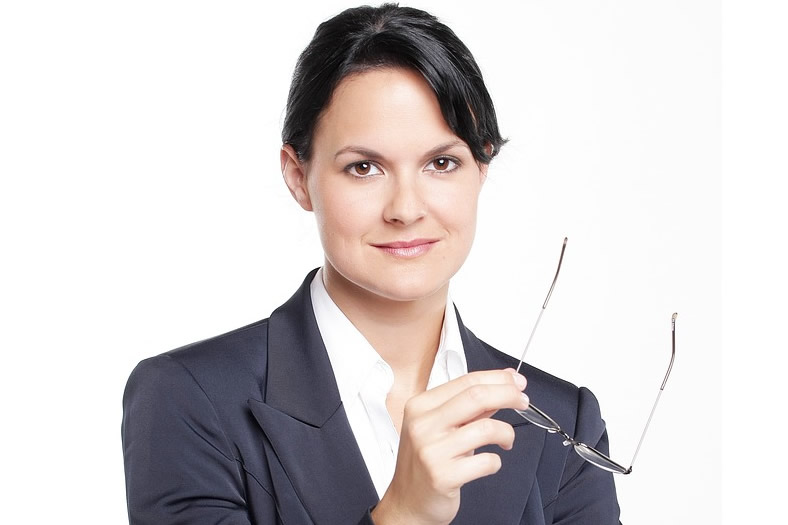
\includegraphics[width=0.5\textwidth,height=\textheight]{img/severina.jpg}
\end{figure}

Severina ha preso il diploma da ragioniera ed è da allora che lavora
nello studio di un commercialista. Ha conosciuto suo marito poco tempo
in una cena aziendale. Hanno avuto una bambina e sono andati a vivere
insieme. Essendo entrambi lavoratori sono stati costretti ad avere una
babysitter per diversi anni. Ora la bambina ha 10 anni e Severina cerca
di passare più tempo possibile con lei.

Anche se la bambina cresce in fretta, lei adora fare shopping per la
piccola: non bada a spese, ma quello che le interessa di più e
l'originalità dei capi. Riserva la ricerca della qualità maggiore per
gli abitini domenicali, insomma le cose che non usa tutti i giorni.
Solitamente compra le taglie per la stagione attuale perché non vuole
vedere la roba tutta ammucchiata nei box o scaffali.

\begin{figure}[h]
\centering
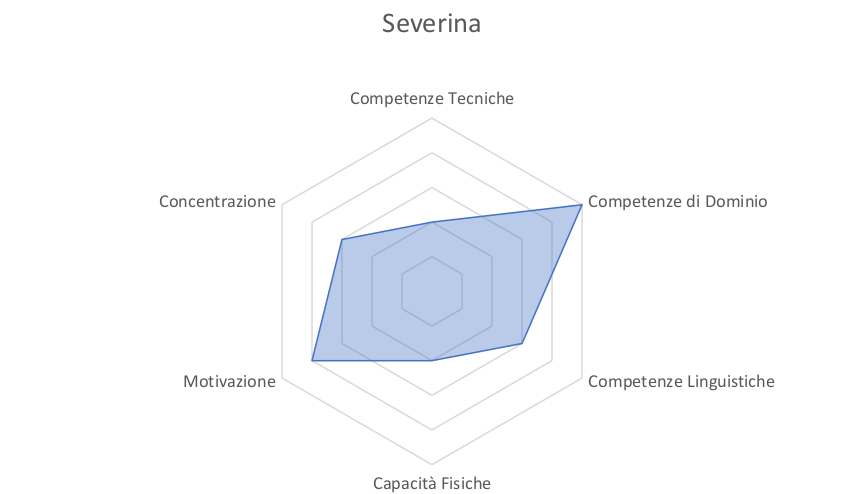
\includegraphics[width=0.7\textwidth,height=\textheight]{img/severina_competenze.png}
\end{figure}

\newpage
\hypertarget{antonio-frastani-1}{%
\subsubsection{Antonio Frastani}\label{antonio-frastani-1}}

\begin{figure}[h]
\centering
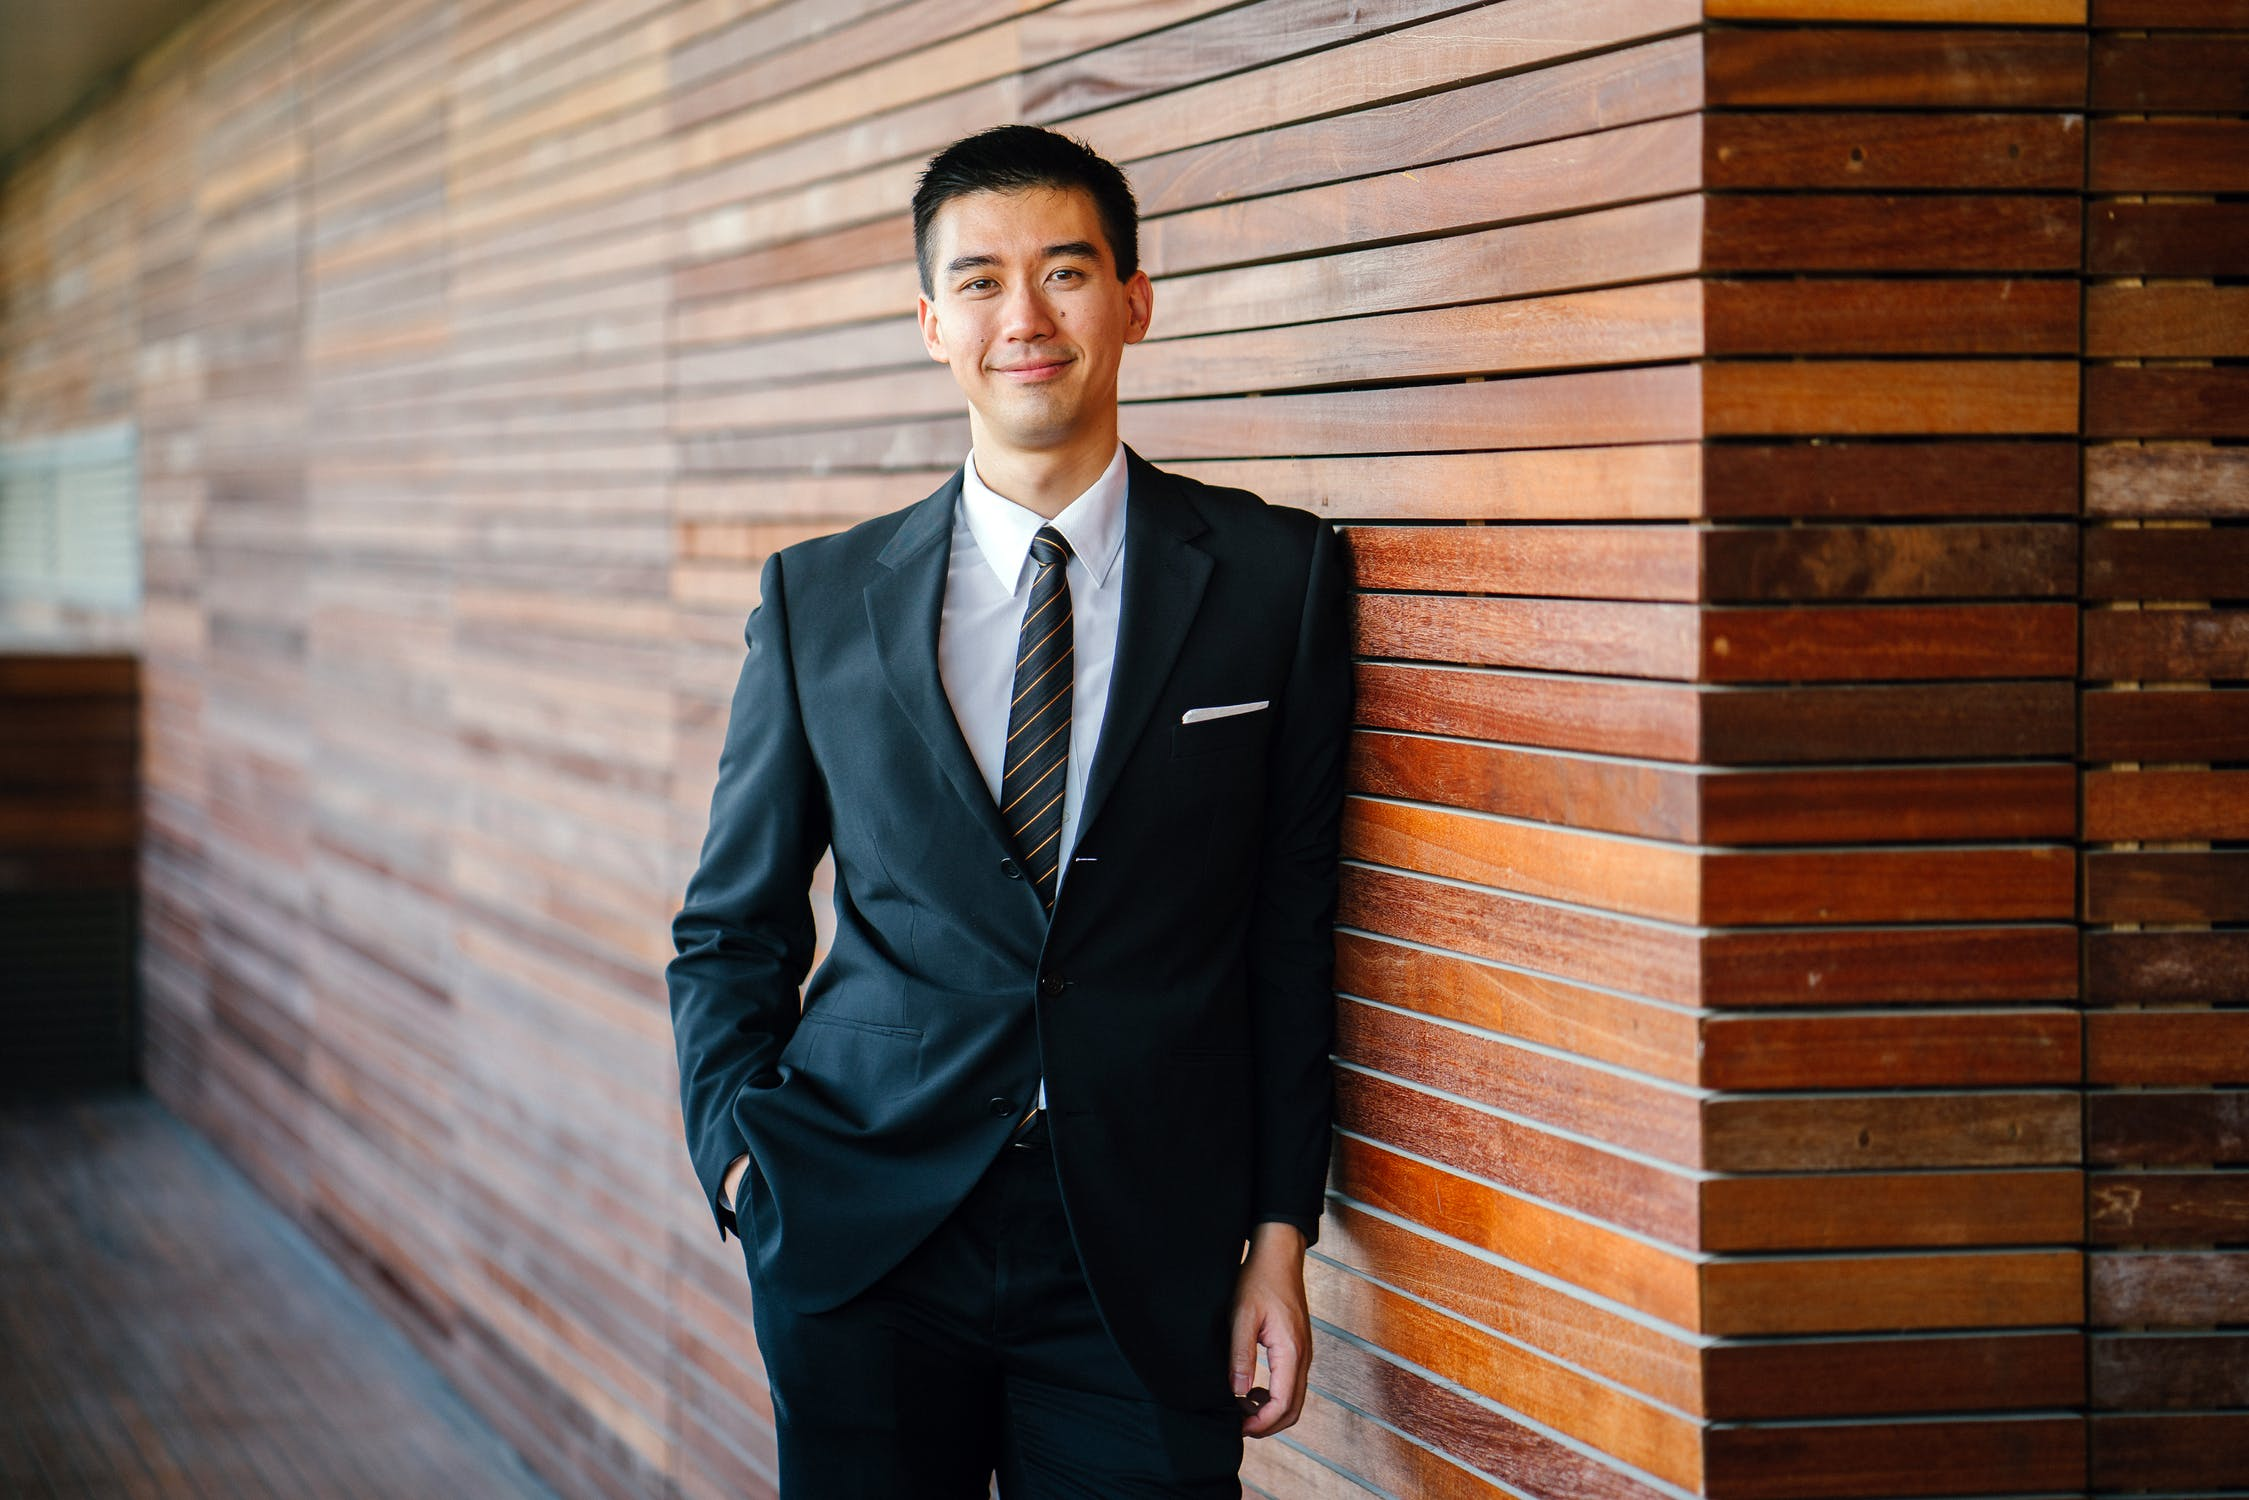
\includegraphics[width=0.5\textwidth,height=\textheight]{img/antonio.jpeg}
\end{figure}

Antonio è un giovane uomo di Firenze. Ha 27 anni e lavora da un anno
circa in una banca locale. Ama il suo lavoro, forse anche grazie allo
stipendio compreso tra i 25K e i 30K. Le sue competenze informatiche
sono ridotte: in ufficio utilizza il PC solo con programmi settoriali e
per redigere documenti, mentre a casa sfrutta il suo iPad Pro 2 per
navigare in rete e visitare i suoi amatissimi social networks. Antonio
adora le macchine e passa quasi tutto il suo tempo libero a vedere
programmi specializzati sull'argomento, raccogliere notizie in rete e
gestisce una pagina Facebook chiamata ``Motori in fiamme''.

\begin{figure}[h]
\centering
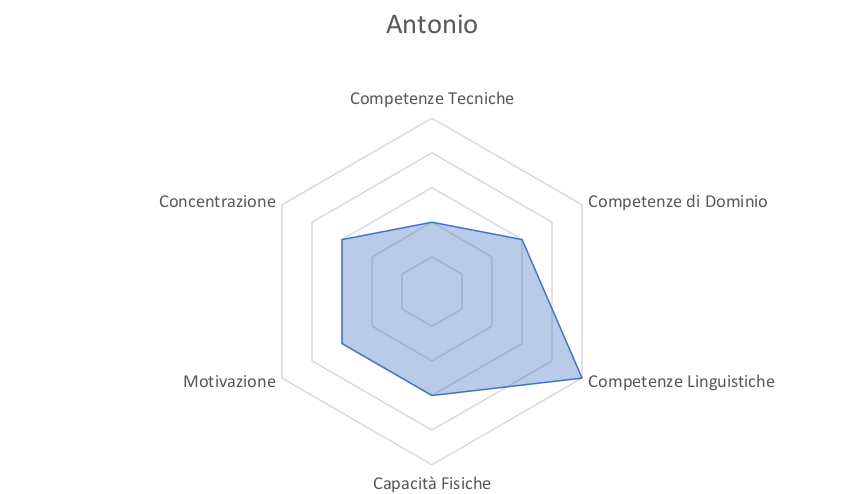
\includegraphics[width=0.7\textwidth,height=\textheight]{img/antonio_competenze.png}
\end{figure}

\newpage
\hypertarget{diego-de-la-vega-1}{%
\subsubsection{Diego de la Vega}\label{diego-de-la-vega-1}}


\begin{figure}[h]
\centering

\includegraphics[width=0.4\textwidth,height=\textheight]{img/diego.jpg}
\end{figure}


Diego ha 26 anni, vive in un appartamento a Trento insieme alla mamma
Adriana di 56 anni, alla sorella Sofia di 28 e al nipotino Pietro di 5
anni. Ha una laurea triennale in Scienze Motorie conseguita
all'università telematica Pegaso.

Lavora da 2 anni nella palestra Body Planet di Trento come personal
trainer. In particolare si occupa di gestire i programmi fitness
individuali dei clienti, motivandoli e guidandoli nel raggiungimento dei
propri obiettivi. Sul posto di lavoro è molto preciso e professionale.
Va d'accordo con tutti i suoi colleghi PT con i quali è solito
scambiarsi consigli e opinioni. Al momento la palestra gli sta pagando
un corso di ginnastica posturale per migliorare la sua preparazione e
renderla più completa. Il suo sport preferito è il basket e non perde
occasione per andare allo stadio a fare il tifo per gli Aquila Basket
Trento.

I suoi obiettivi sono di riuscire ad aprire una palestra in cui
insegnare e applicare le tecniche dell'allenamento funzionale e di
trasferirsi a vivere da solo in un appartamento nella periferia
torinese, lontano dal traffico e dalla confusione della metropoli.

Diego utilizza il computer ogni giorno, sia al lavoro, per tenere
monitorata tutta l'attività riguardante i clienti, dalle schede di
allenamento, alla fatturazione, tramite l'applicativo PT Software 2.0,
sia a casa, per studiare, giocare, fare ricerche e molto altro. Per
quanto riguarda lo smartphone, l'unico uso che ne fa è per gestire i
suoi profili social. Percepisce uno stipendio lordo annuo di 25000 €.

\begin{figure}[h]
\centering
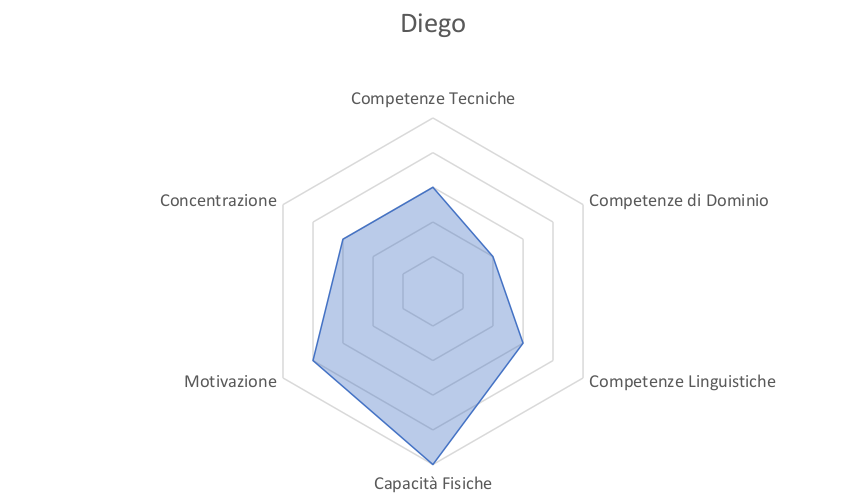
\includegraphics[width=0.7\textwidth,height=\textheight]{img/diego_competenze.png}
\end{figure}


\hypertarget{elisa-pezzana-1}{%
\subsubsection{Elisa Pezzana}\label{elisa-pezzana-1}}

\begin{figure}[h]
\centering

\includegraphics[width=0.5\textwidth,height=\textheight]{img/elisa.jpg}
\end{figure}

Elisa, 32 anni, ha studiato economia a Bologna e dopo un paio di anni dalla laurea
ha vinto il concorso di segretaria comunale nel comune di residenza, è
sposata da 15 anni con Giorgio e hanno due figli. Elisa è una donna
solare, socievole e simpatica. Dimostra qualche anno in meno rispetto
alla sua età e le piace nuotare e cucinare Obiettivi: Organizzare le
vacanze estive con la famiglia.

Elisa il lunedi e il mercoledi va in palestra, il giovedi fa pilates con
le amiche e il martedi e venerdi va in piscina. La domenica mattina ha
l'abitudine di andare a fare colazione con le amiche al bar in centro
città.

\begin{figure}[h]
\centering
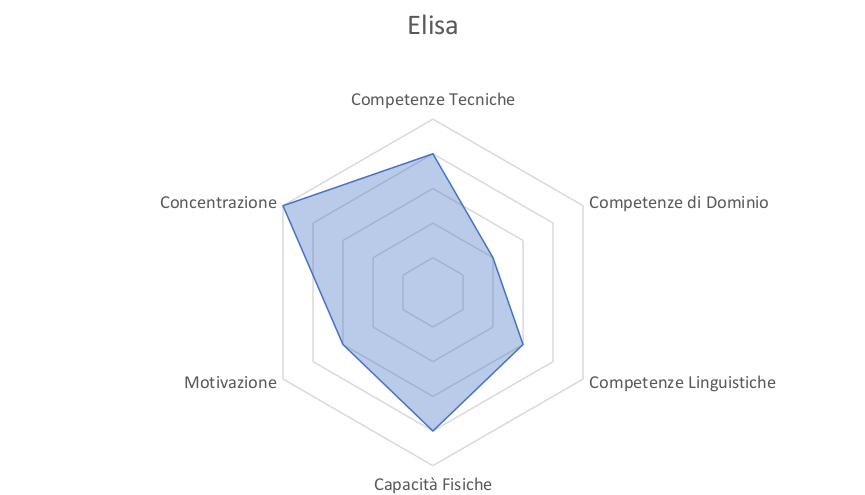
\includegraphics[width=0.7\textwidth,height=\textheight]{img/elisa_competenze.png}
\end{figure}

\subsubsection{Giorgia Moro}\label{giorgia-moro-1}



Giorgia ha 38 anni, vive in un modesto appartamento a pochi chilometri
dal centro di Torino insieme alla sua famiglia. Ha una laurea triennale
in Economia e Commercio conseguita presso l'Università di Bologna. È
sposata con Andrea e hanno una figlia, Alice, di 8 anni.

\begin{figure}[h]
\centering

\includegraphics[width=0.5\textwidth,height=\textheight]{img/giorgia.jpg}
\end{figure}

Lavora da undici anni all'interno di un rinomato studio legale, operante
sia in Italia che all'estero, come impiegata contabile dove percepisce
uno stipendio lordo annuo di 36000€. Svolge il suo lavoro a stretto
contatto con gli altri membri dello studio, con i quali si confronta e
si scambiano idee, consigli e suggerimenti.

Utilizza raramente il PC, quasi esclusivamente per leggere email di
lavoro e guardare ricette da preparare per la famiglia. Ha una
certificazione di inglese di livello C1 conseguita al British Institutes
di Bologna, durante gli anni universitari, che le garantisce sia
un'ottima comprensione della lingua scritta e parlata sia un'ottima
capacità di scrittura. Da circa 3 mesi lo studio le sta pagando un corso
online sul GDPR.

Quando non lavora, a Giorgia piace navigare in rete con il suo
smartphone e tenere sempre aggiornato il suo profilo Facebook e
Instagram. Da diversi anni ha un abbonamento online a Vanity Fair,
attraverso il quale si tiene aggiornata sulle ultime tendenze. Nel tempo
libero le piace andare a visitare i mercatini d'antiquariato nella
periferia torinese, insieme alla figlia Alice, per cercare oggetti unici
e originali.

L'obiettivo di Giorgia è di comprare un nuovo appartamento, più grande e
più vicino al centro di Torino, e arredarlo con mobili e oggetti
d'antiquariato.

\begin{figure}[h]
\centering
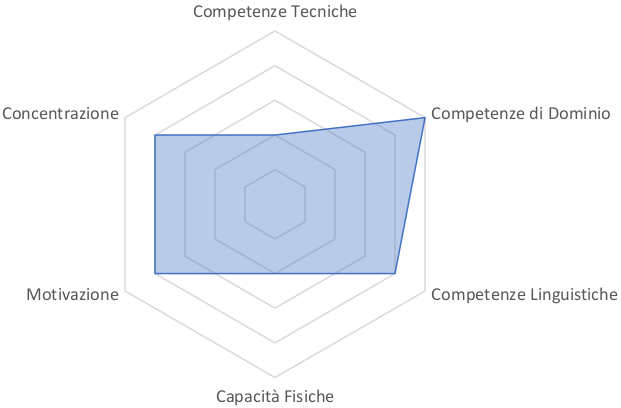
\includegraphics[width=0.7\textwidth,height=\textheight]{img/giorgia_competenze.png}
\end{figure}

\hypertarget{operazioni}{%
\subsection{Operazioni}\label{operazioni}}

Nel modello CAO=S, le operazioni riguardano la manipolazione dei concetti, elencati nella sezione precedente. La tipologia di operazioni considerate sono quelle comunemente definite \emph{CRUD}: \emph{Create}, \emph{Read}, \emph{Update} e \emph{Delete}. Questo significa analizzare le modalità di creazione, lettura, aggiornamento e rimozione dei concetti elencati.

Ogni operazione è caratterizzata da determinate proprietà:

\subsubsection{Creazione}\label{creazione}

\begin{itemize}
\tightlist
\item
  \textbf{Tipo}: la creazione può essere manuale, se avviene tramite un
  interazione con l'utente, automatica se è il sistema stesso ad
  aggiungere un elemento o implicita se viene eseguita dagli
  amministratori
\item
  \textbf{Valori di default}: lo stato iniziale con il quale un concetto
  viene valorizzato nel momento in cui viene aggiunto
\item
  \textbf{Moltiplicità}: singola o multipla a seconda della quantità di
  istanze che il sistema permette di inserire in una sola volta
\item
  \textbf{Persistenza}: indica la capacità di persistere o meno un
  istanza all'interno del sistema una volta che è stata aggiunta
\item
  \textbf{Memoria dell'utente}: in aggiunta ai valori di default, indica
  la presenza o meno di suggerimenti dati in base a valori inseriti in
  precedenza
\item
  \textbf{Notifiche di fallimento}: in caso di fallimento
  dell'operazione di salvataggio (funzione disponibile solo per l'utente loggato) indica se è presente o meno un
  messaggio di errore.
\end{itemize}

\hypertarget{lettura}{%
\subsubsection{Lettura}\label{lettura}}

\begin{itemize}
\tightlist
\item
  Vista individuale \textbf{completa}: il concetto è visualizzato
  singolarmente in ogni suo dettaglio.
\item
  Vista individuale \textbf{ridotta}: i concetti sono visualizzati
  singolarmente e solo una parte delle loro informazioni è visibile
\item
  Vista \textbf{multipla}: permette la visualizzazione di più concetti
  contemporaneamente. Può essere una lista, che permette di visualizzare
  poche informazioni per ogni concetto, una lookup, attraverso la quale
  è possibile selezionare uno o più concetti per un uso futuro o un
  riassunto, usato per mostrare una descrizione non dettagliata di ogni
  concetto esposto
\end{itemize}

\hypertarget{aggiornamento}{%
\subsubsection{Aggiornamento}\label{aggiornamento}}

\begin{itemize}
\tightlist
\item
  \textbf{Globale}: tutte le proprietà di una determina istanza sono
  modificabili
\item
  \textbf{Specifico}: solo alcune delle proprietà di una determinata
  istanza sono modificabili
\end{itemize}

\hypertarget{eliminazione}{%
\subsubsection{Eliminazione}\label{eliminazione}}

\begin{itemize}
\tightlist
\item
  \textbf{Eliminazione}: l'entità viene completamente eliminata e non è
  più presente all'interno del sistema
\item
  \textbf{Archiviazione}: l'entità non viene del tutto eliminata, può
  essere ripristinata o eliminata definitivamente
\end{itemize}

Il progetto proposto è un sottosito di contenuti, quindi le operazioni effettuabili dagli attori principali sono di creazione, visualizzazione, aggiornamento ed eliminazione. Le operazioni di visualizzazione, aggiornamento ed eliminazione sono disponbili anche nel sito di riferimento kiabi.it, ma su concetti e con modalità differenti.

\begin{longtable}[]{lllll}
\toprule
\begin{minipage}[b]{0.17\columnwidth}\raggedright
\strut
\end{minipage} & \begin{minipage}[c]{0.17\columnwidth}\raggedright
Creazione\strut
\end{minipage} & \begin{minipage}[c]{0.17\columnwidth}\raggedright
Vista\strut
\end{minipage} & \begin{minipage}[c]{0.27\columnwidth}\raggedright
Aggiornamento\strut
\end{minipage} & \begin{minipage}[c]{0.17\columnwidth}\raggedright
Eliminazione\strut
\end{minipage}\tabularnewline
\midrule
\endhead
\begin{minipage}[t]{0.17\columnwidth}\raggedright
Modello\strut
\end{minipage} & \begin{minipage}[t]{0.17\columnwidth}\raggedright
Creazione di una maglietta personalizzata\strut
\end{minipage} & \begin{minipage}[t]{0.17\columnwidth}\raggedright
Maglietta durante la personalizz.\strut
\end{minipage} & \begin{minipage}[t]{0.17\columnwidth}\raggedright
Modifica di una maglietta durante la personalizz.\strut
\end{minipage} & \begin{minipage}[t]{0.17\columnwidth}\raggedright
Sì\strut
\end{minipage}\tabularnewline
\begin{minipage}[t]{0.17\columnwidth}\raggedright
Progetti personali\strut
\end{minipage} & \begin{minipage}[t]{0.17\columnwidth}\raggedright
No\strut
\end{minipage} & \begin{minipage}[t]{0.17\columnwidth}\raggedright
Sì\strut
\end{minipage} & \begin{minipage}[t]{0.17\columnwidth}\raggedright
Sì\strut
\end{minipage} & \begin{minipage}[t]{0.17\columnwidth}\raggedright
Sì\strut
\end{minipage}\tabularnewline
\begin{minipage}[t]{0.17\columnwidth}\raggedright
Catalogo\strut
\end{minipage} & \begin{minipage}[t]{0.17\columnwidth}\raggedright
No\strut
\end{minipage} & \begin{minipage}[t]{0.17\columnwidth}\raggedright
Sì\strut
\end{minipage} & \begin{minipage}[t]{0.17\columnwidth}\raggedright
Votazione positiva o negativa di un progetto\strut
\end{minipage} & \begin{minipage}[t]{0.17\columnwidth}\raggedright
No\strut
\end{minipage}\tabularnewline
\begin{minipage}[t]{0.17\columnwidth}\raggedright
Più votati\strut
\end{minipage} & \begin{minipage}[t]{0.17\columnwidth}\raggedright
No\strut
\end{minipage} & \begin{minipage}[t]{0.17\columnwidth}\raggedright
Sì\strut
\end{minipage} & \begin{minipage}[t]{0.17\columnwidth}\raggedright
No\strut
\end{minipage} & \begin{minipage}[t]{0.17\columnwidth}\raggedright
No\strut
\end{minipage}\tabularnewline
\bottomrule
\end{longtable}

\subsection{Strutture}\label{strutture}

Una volta identificati gli utenti, i concetti e le operazioni, il passo
successivo di CAO=S consiste nella definizione delle strutture. Questo
avviene tramite la compilazione di tabelle tridimensionali che mostrano
come gli attori interagiscono con i vari concetti usando le operazioni
descritte.

La tabella ha per assi i concetti, gli attori e le operazioni. All'interno di ogni cella si inseriscono delle annotazioni di come un attore deve poter eseguire l'operazione sul quel determinato concetto.

Ci sono tre tipi di strutture che interessano lo sviluppo:

\begin{itemize}
\tightlist
\item
  \textbf{Viste}: maschere di visualizzazione delle proprietà dei
  concetti
\item
  \textbf{Navigazione}: meccanismi di passaggio da una vista all'altra
\item
  \textbf{Strutture dati}: normalizzazione dello studio dei concetti in
  modelli di memorizzazione persistente delle entità
\end{itemize}

\begin{longtable}[]{lllll}
\toprule
Concetti & Creazione & Vista & Aggiornamento &
Eliminazione\tabularnewline
\midrule
\endhead
Modello & Editor & Dettaglio & Editor & Editor\tabularnewline
Catalogo & No & Multipla & Votazione di un progetto, Editor & No\tabularnewline
Progetti personali & No & Multipla & Votazione di un progetto, Editor & Sì\tabularnewline
Più votati & No & Multipla & Editor & No\tabularnewline
\bottomrule
\end{longtable}

\hypertarget{progettazione-dellinterazione}{%
\section{Progettazione
dell'interazione}\label{progettazione-dellinterazione}}

Lo scopo dell'applicazione è quello di fornire agli utenti uno store
online dove possano personalizzare una t-shirt ed avere la possibilità
di riceverla a casa.

L'interazione può essere vista come un dialogo tra utente e computer. La
scelta dello stile di interazione ha profondi effetti sulla natura del
dialogo e, di conseguenza, sull'efficacia dell'interazione.

Sono stati identificati sei principali stili di interazione:

\begin{itemize}
\tightlist
\item
  \textbf{Menu and navigation}
\item
  \textbf{Command entry}
\item
  \textbf{Question/Answer}
\item
  \textbf{Spreadsheet/form-fill}
\item
  \textbf{Natural language}
\item
  \textbf{Direct manipulation}
\end{itemize}

Ai fini del progetto é stato utilizzato principalmente lo stile ``Menu e
navigazione''. Esso permettere di organizzare i comandi in menu
gerarchici risolvendo il problema della visualizzazione di questi che,
quando numerosi, possono arrivare ad occupare una grossa parte dello
schermo.

Anche se questo tipo di interazione potrebbe rallentare gli utenti
esperti, in realtà, data la presenza di un numero di categorie e
sottocategorie limitate non impatta sulla velocità di esecuzione delle
operazioni.

Per quanto riguarda la disposizione fisica dei controlli si è deciso di
adottare un approccio con raggruppamenti funzionali, ossia sono stati
raggruppati insieme i comandi che permettono interazioni correlate.

Per quanto riguarda la navbar in alto, sono presenti due sezioni.

La prima sezione appartiene al sito madre Kiabi e contiene:

\begin{itemize}
\tightlist
\item
  Logo: permette di identificare il sito ed ha un link che consente di
  tornare sempre alla pagina principale;
\item
  Barra di ricerca: permette di effettuare una query in linguaggio
  naturale per cercare tra gli articoli presenti nel catalogo. Vengono
  utilizzate tecniche come la query expansion per ampliare l'output di
  ricerca con sinonimi delle parole ricercate. Il risultato sarà una
  lista di articoli che soddisfano le richieste della query;
\item
  Profilo: permette l'accesso rapido alle informazioni dell'account,
  alle modalità di pagamento, agli ordini effettuati (appartiene a Kiabi);
\item
  Whishlist: permette di salvare gli articoli di interesse senza
  caricarli nel carrello (appartiene a Kiabi);
\item
  Carrello: permette di accedere alla lista di articoli pronti per
  essere acquistati (appartiene a Kiabi);
\end{itemize}

La seconda sezione contiene il menu di navigazione e varia in funzione
della tipologia di utente. Per l'utente non loggato offre:

\begin{itemize}
\tightlist
\item
  Home: permette di accedere alla pagina principale del sottosito
\item
  Catalogo: permette di accedere al catalogo con la lista dei prodotti
  già personalizzati da tutti gli utenti
\item
  Più Votati: permette di accedere alla lista dei podotti più votati
\end{itemize}

Per l'utente loggato, oltre alle aree precedenti, si aggiunge:

\begin{itemize}
\tightlist
\item
  Progetti Personali: permette di accedere alla lista di prodotti   personalizzati dall'utente stesso
\end{itemize}

Esiste una ulteriore barra posta in basso che viene visualizzata solo quando si è all'interno dell'editor. Essa ospita i link rapidi che permettono di acquistare un prodotto (aggiungendolo al carrello) o di salvarlo nei progetti personali. Inoltre ospita un drop-up menu con la lista delle modifiche selezionate.

Nella schermata principale dell'editor, sulla parte sinistra, sono presenti quattro miniature che descrivono le macrocategorie personlizzabili: colletto, busto, maniche e taglia. All'interno di ognuna di queste categorie è presente un menù a schede che contiene tutte le possibili personalizzazioni per quella specifica area della maglietta. 

Il footer (in basso) contiene informazioni sui contatti (telefono ed e-mail), varie informazioni su pagamenti, modalità di spedizione, aiuto, FAQ e informazioni. Esso fa parte del sito madre Kiabi.

\newpage
\hypertarget{blueprints}{%
\section{Blueprints}\label{blueprints}}

Le blueprint sono semplici diagrammi che definiscono l'organizzazione dei contenuti e come le varie componenti interagiscono tra di loro.

Saranno presentate tre blueprint che mostrano rispettivamente:

\begin{enumerate}
\def\labelenumi{\arabic{enumi}.}
\item
  Organizzazione dei contenuti disponibili per un utente loggato (Fig. \ref{utente loggato})
\item
  Organizzazione dei contenuti disponibili per un utente non loggato (Fig. \ref{utente non loggato})
\item
  Creazione di un nuovo modello (Fig. \ref{creazione modello})
\end{enumerate}

\begin{figure}[h]
\centering
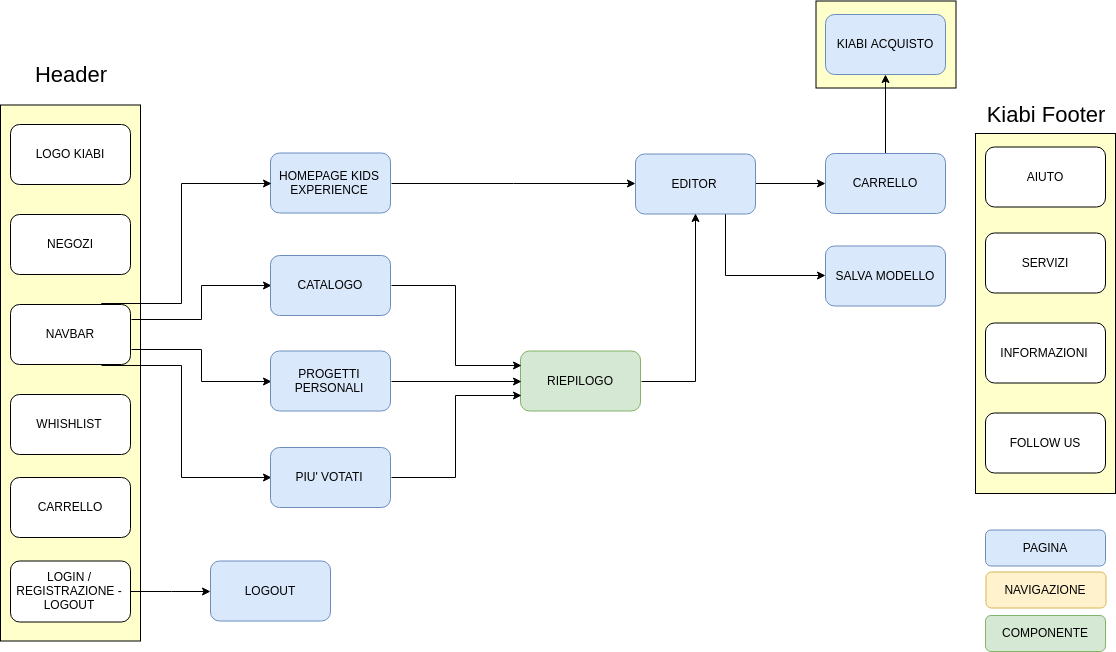
\includegraphics[width=0.8\textwidth]{img/Utente_loggato.png}
\caption{Contenuti disponibili - Utente loggato}
\label{utente loggato}
\end{figure}

\begin{figure}[h]
\centering
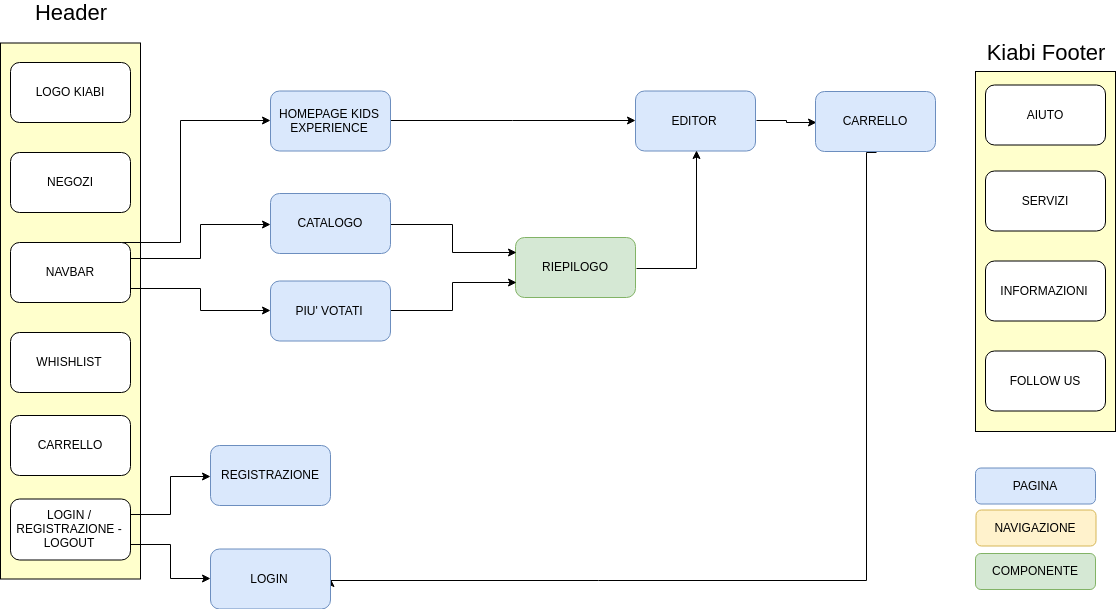
\includegraphics[width=0.8\textwidth]{img/Utente_non_loggato.png}
\caption{Contenuti disponibili - Utente non loggato}
\label{utente non loggato}
\end{figure}

\begin{figure}[h]
\centering
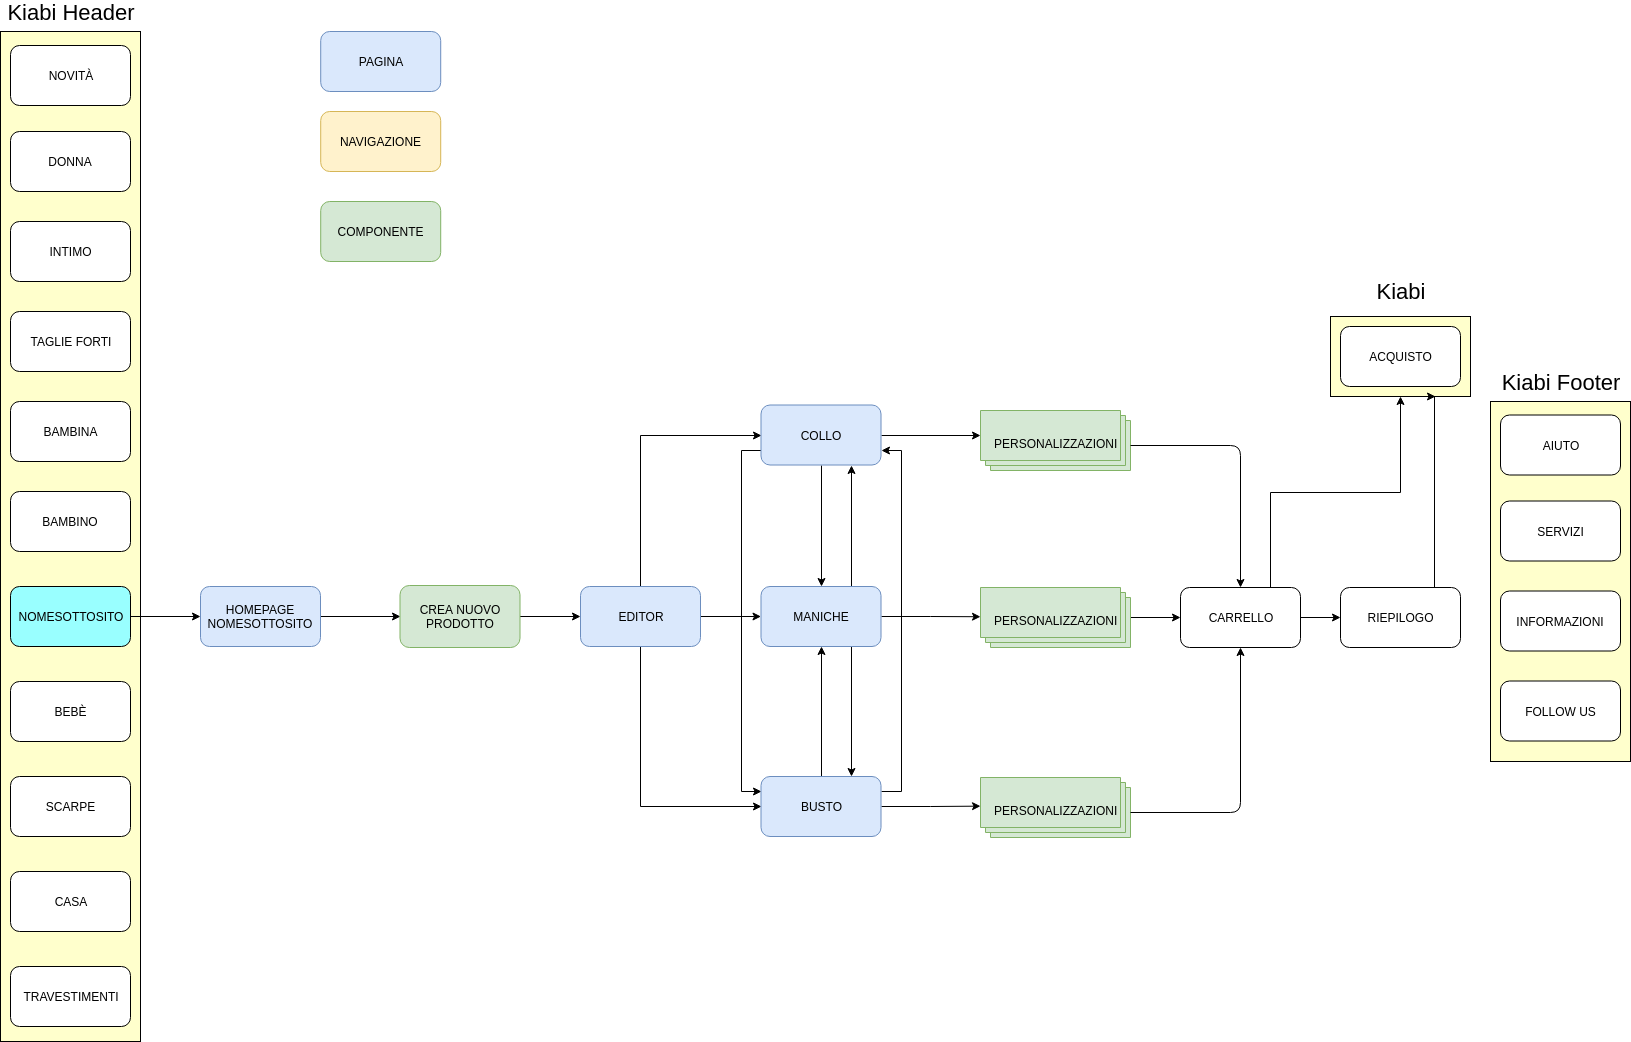
\includegraphics[width=0.8\textwidth]{img/Creazione_modello.png}
\caption{Creazione modello}
\label{creazione modello}
\end{figure}

\newpage
\section{Wireframes}\label{wireframes}

I wireframe sono illustrazioni organizzative schematiche dei contenuti
presenti in un progetto. La funzione principale dei wireframe è di
comunicare l'idea del progetto, focalizzando l'attenzione
sull'architettura piuttosto che il design. Contengono i comandi
necessari per permettere all'utente di realizzare un task. Spesso sono
anche accompagnati da testo e immagini. 

Sono strumenti potenti che
permettono di effettuare test con gli utenti per la valutazione del
sistema e permettono di apportare modifiche restando ancora in fase di
prototipazione con conseguente risparmi di tempo e denaro.

\subsection{Home}\label{home}

La Home di Kids Experience è divisa in tre sezioni: header, corpo e footer. La pagina è scrollabile e l'header rimane sempre visibile in quanto contiene elementi che garantiscono un accesso rapido alle altre sezioni.

Il corpo ha una funzione prevalentemente informativa. Di fondamentale importanza sono lo slogan e il bottone ``Crea!'' che permette un accesso diretto all'editor.

Il footer, ereditato da Kiabi, contiente elementi marginali di navigazione come: una sezione di aiuto, una di servizi, una sezione informativa e i rimandi ai principali social network.

\begin{figure}[h]
\centering
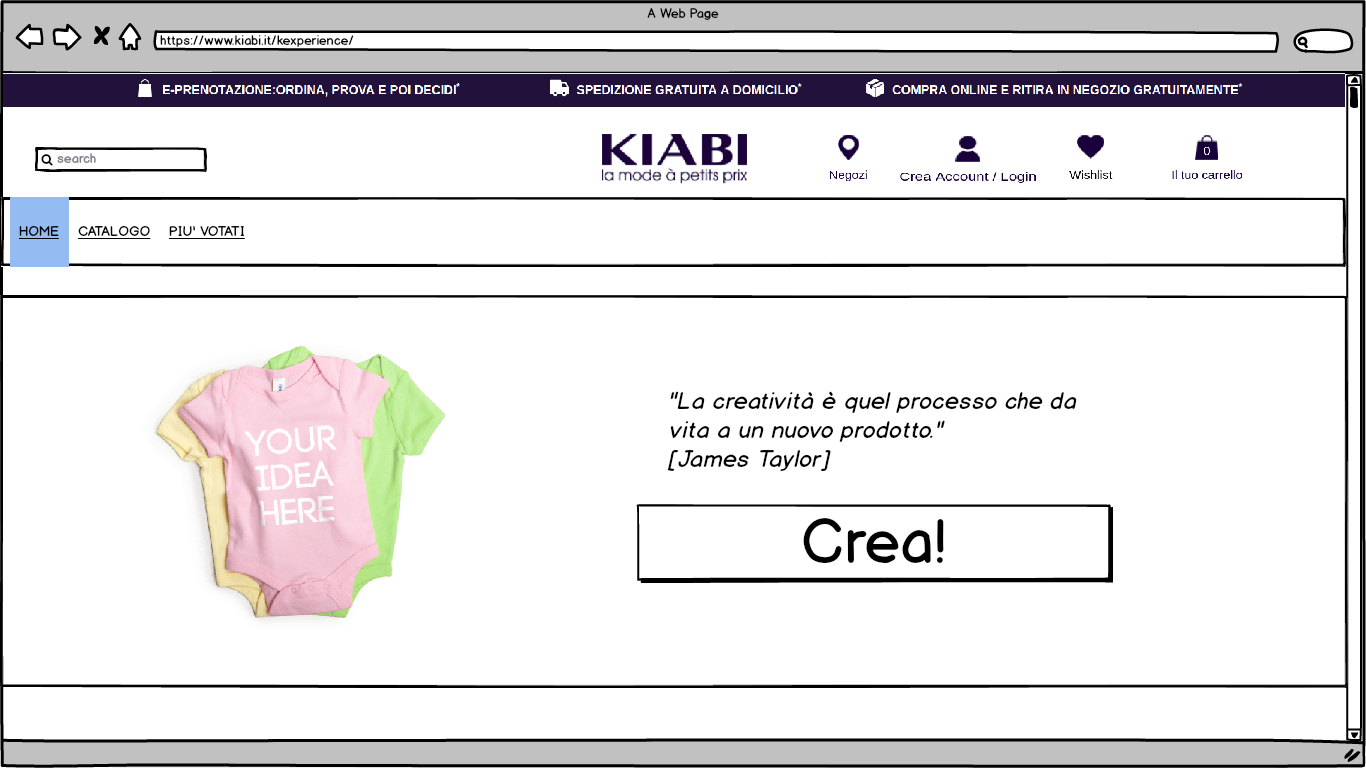
\includegraphics[width=0.9\textwidth]{../balsamiq/balsamiq_finale/HomeSottositoUtenteEsterno.png}
\caption{Home Kids Experience}
\end{figure}

\newpage
\subsection{Creazione modello}\label{creazione-modello}

Il processo di creazione di una maglietta personalizzata si compone di svariati passaggi data l'ampia gamma di personalizzazioni disponibili.
Sulla parte sinistra della schermata sono presenti le quattro
macrocategorie di personalizzazioni. Dall'altro lato è presentata un'anteprima in tempo reale delle personalizzazioni applicate e una miniatura che permette di invertire il lato visibile della maglietta, permettendo una personalizzazione a 360°.

Tramite i link sulla sinistra è possibile accedere alle finestre di dettaglio delle personalizzazioni. In ogni sezione dell'editor è presente una navbar che permette un rapido accesso alle sezioni principali di Kids Experience. Infine nell'header è presente una comoda barra di ricerca che permette di cercare risultati sia nel catalogo di Kiabi che
in quello di Kids Experience.

\begin{figure}[h]
\centering
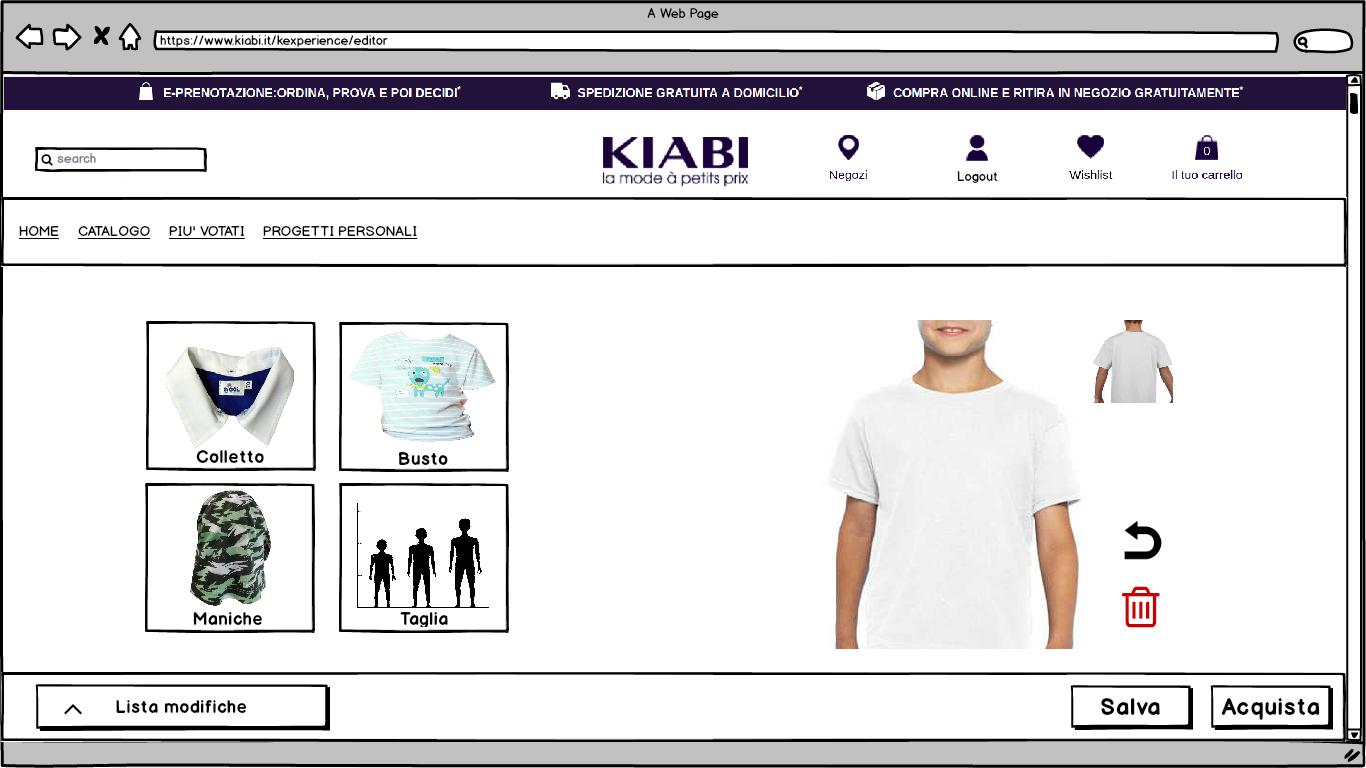
\includegraphics[width=0.9\textwidth]{../balsamiq/balsamiq_finale/Editorbase.png}
\caption{Editor}
\end{figure}

Ogni volta che viene inserita una personalizzazione, oltre ad essere visualizzata direttamente sul modello, appare anche all'interno della lista delle modifiche, insieme al costo unitario ed un'icona per la rimozione. Il costo totale della maglietta e delle personalizzazioni applicate è sempre ben visibile nella barra in basso.
Nella medesima barra sono presenti i bottoni per salvare il progetto attuale nei progetti personali o per acquistarlo.

\begin{figure}[h]
\centering
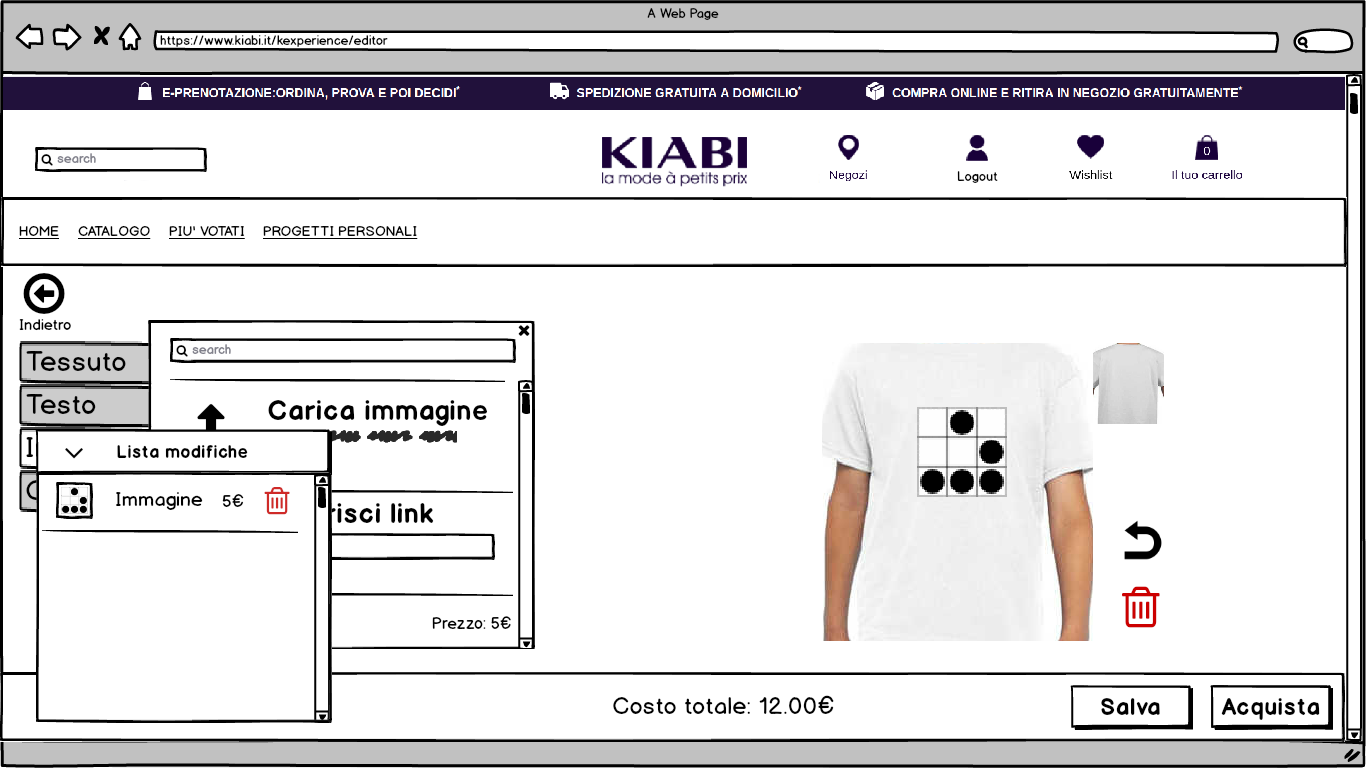
\includegraphics[width=0.9\textwidth]{../balsamiq/balsamiq_finale/Editor-caratteristicabustoimmagine4.png}
\caption{Editor - Inserimento immagine}
\end{figure}

\begin{figure}[h]
\centering
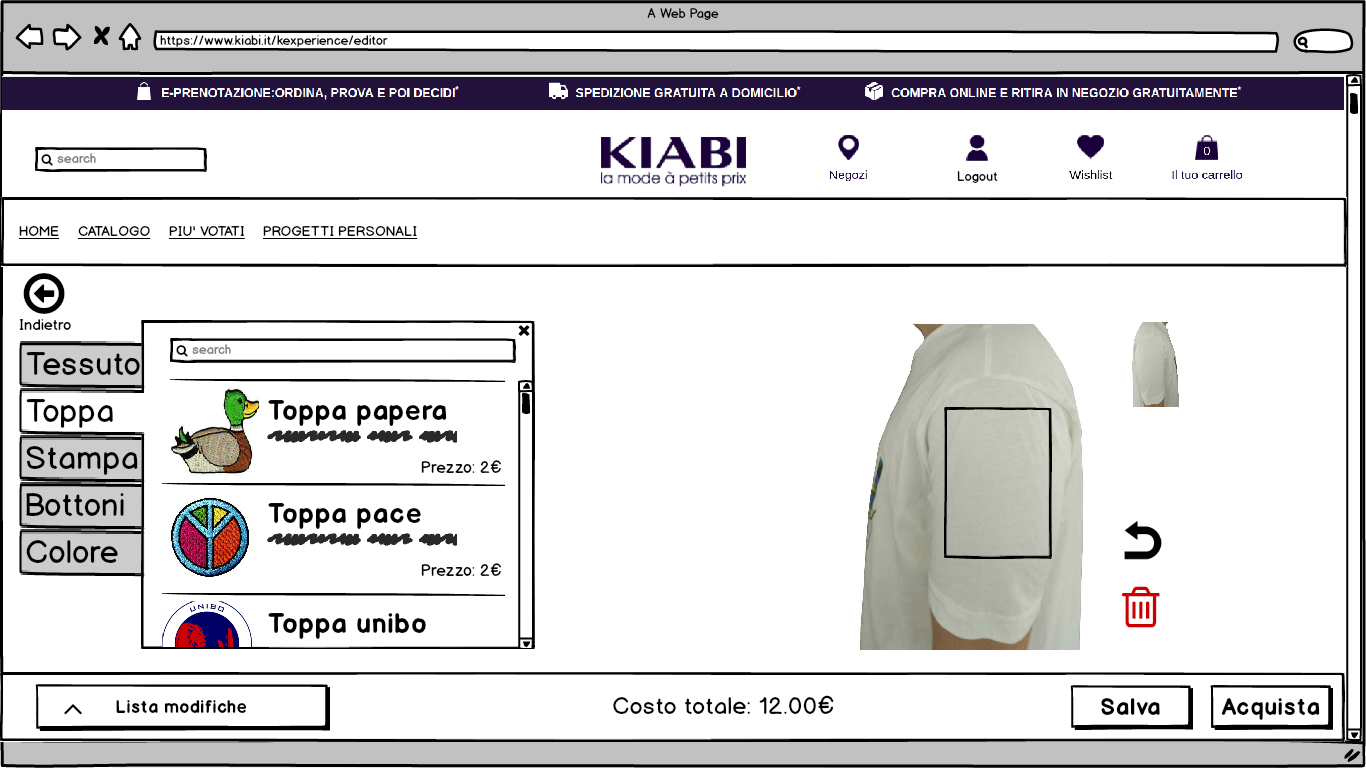
\includegraphics[width=0.9\textwidth]{../balsamiq/balsamiq_finale/Editor-caratteristicamanichetoppa.png}
\caption{Editor - Search bar}
\label{searchbar}
\end{figure}

\begin{figure}[h]
\centering
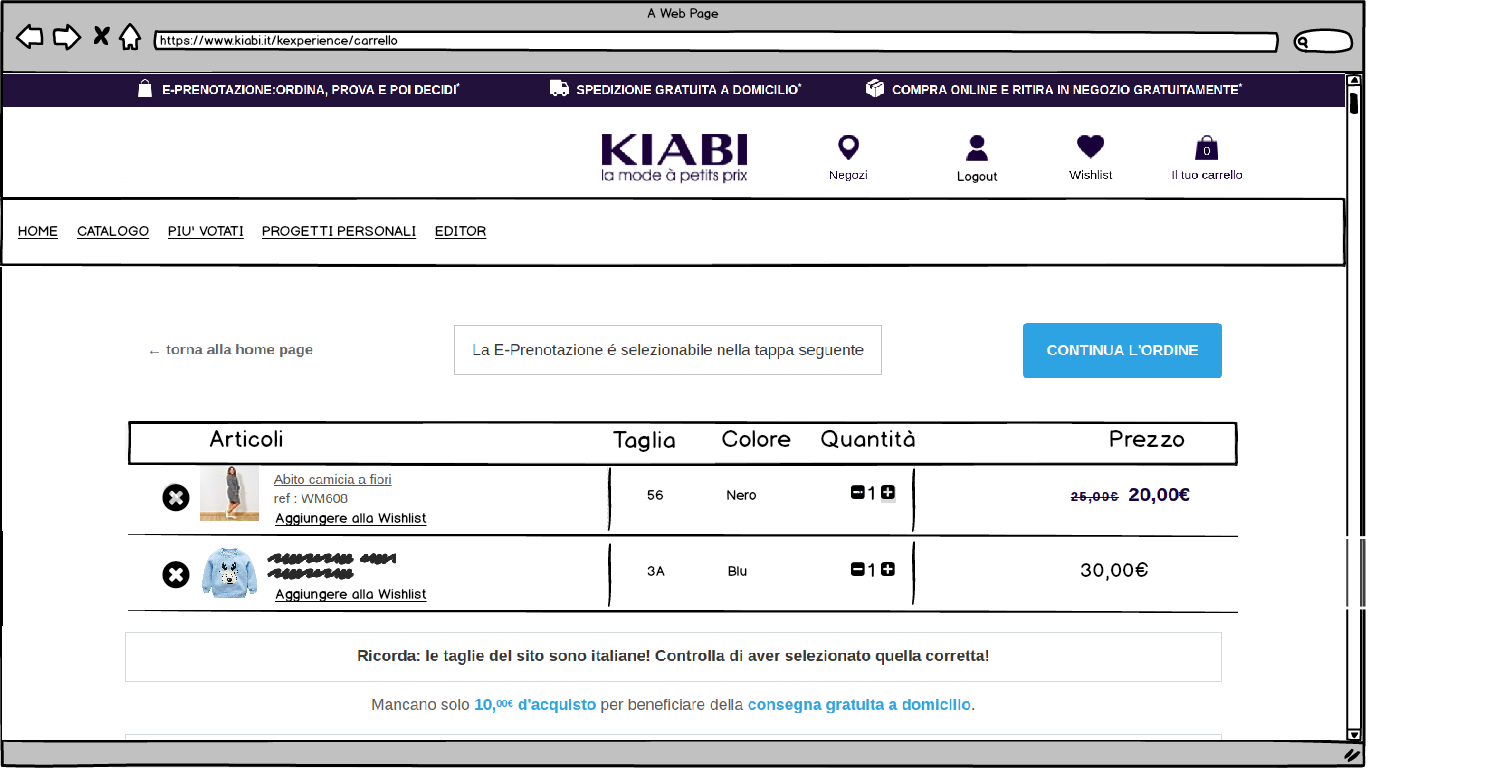
\includegraphics[width=0.9\textwidth]{../balsamiq/balsamiq_finale/Carrello.png}
\caption{Carrello}
\label{carrello}
\end{figure}

Nel menù in cui vengono mostrate le varie personalizzazioni, è presente anche una comoda search bar (Fig. \ref{searchbar}) che permette, tramite query in linguaggio naturale, di cercare direttamente il tipo di personalizzazione richiesta.

Procendo con l'acquisto si giunge nella pagina del carrello (Fig. \ref{carrello}). Qui
troviamo un riepilogo dei prodotti inseriti finora, con la possibilità
di modificarne il numero di pezzi.


\begin{figure}[ht]
\centering
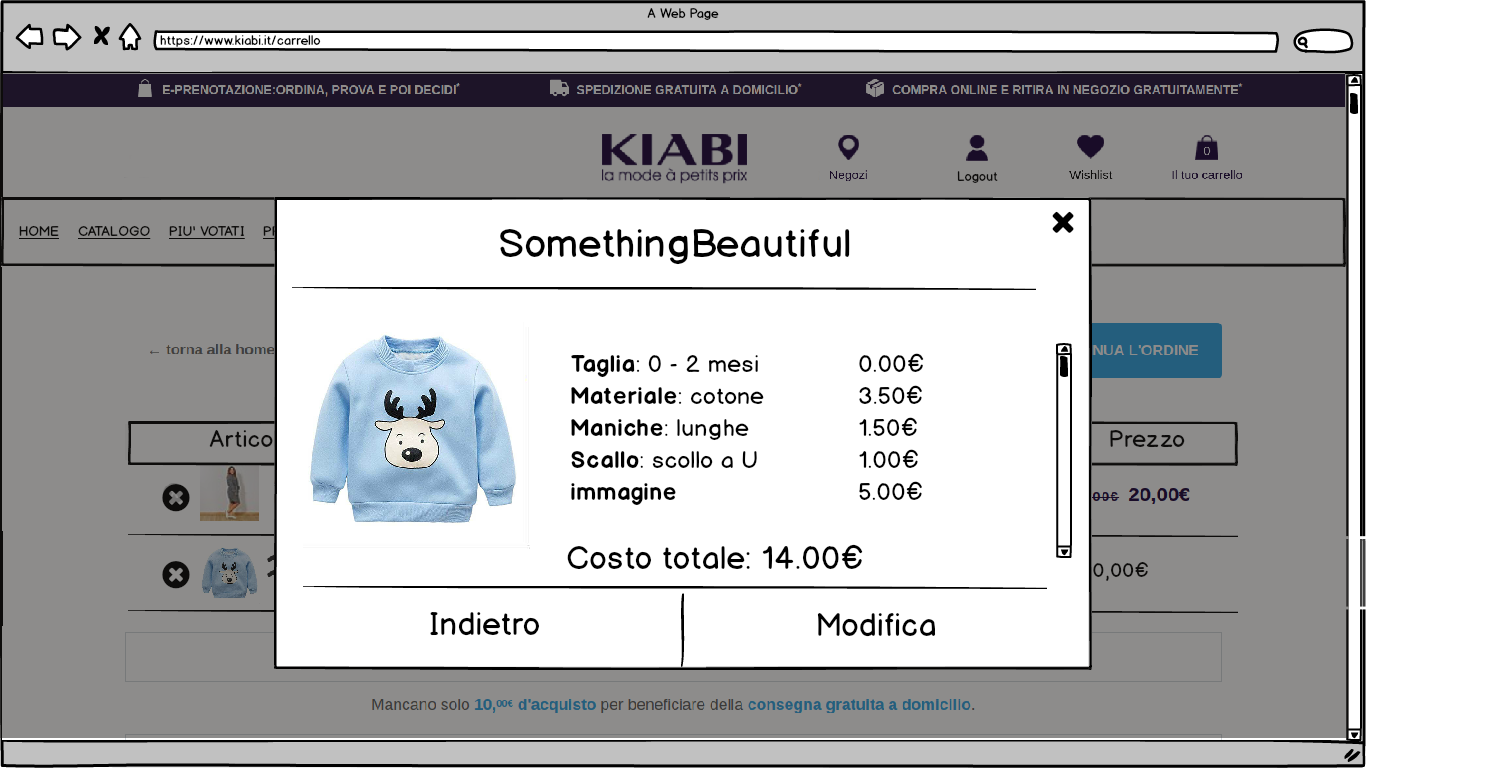
\includegraphics[width=0.9\textwidth]{../balsamiq/balsamiq_finale/Carrellodettagli.png}
\caption{Carrello - dettaglio}
\label{carr-dett}
\end{figure}

Premendo sulla miniatura di uno dei prodotti presenti nel carrello si
apre un modale (Fig. \ref{carr-dett}) in cui è presente una lista completa delle
personalizzazioni e relativi costi, il costo totale e un bottone che
permette di tornare all'editor per continuare la personalizzazione.



\newpage
\hypertarget{catalogo}{%
\subsection{Catalogo}\label{catalogo}}

\begin{figure}[h]
\centering
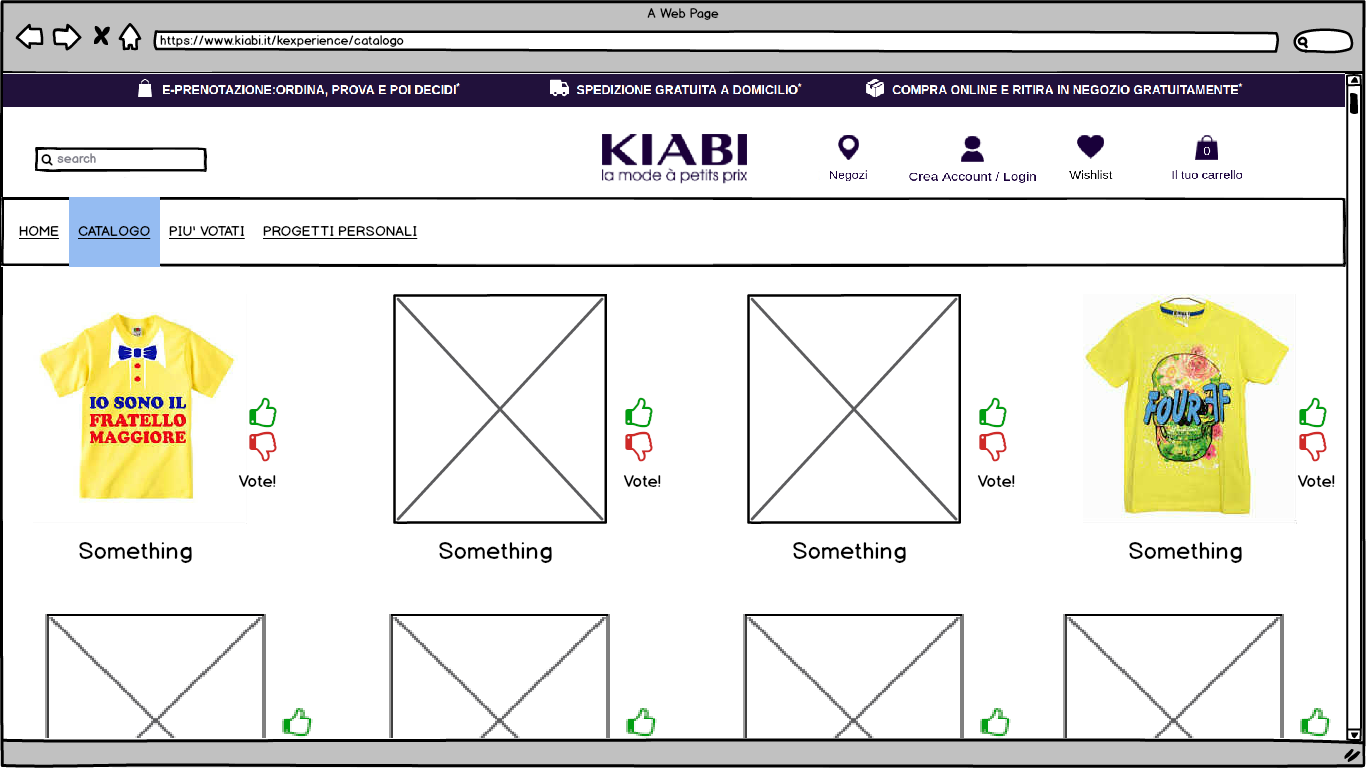
\includegraphics[width=0.9\textwidth]{../balsamiq/balsamiq_finale/Catalogo.png}
\caption{Catalogo}
\label{catalogo}
\end{figure}

Il catalogo (Fig. \ref{catalogo}) è una delle sezioni principali e contiene al suo interno tutte le creazioni degli utenti che hanno deciso di salvarle, ordinate per data di creazione.

Premendo su una singola maglietta viene mostrato un modale riepilogativo (Fig. \ref{cat-dett})
che contiene costo totale della maglietta, l'elenco delle
personalizzazioni applicate e il nome dell'autore.

\begin{figure}[h]
\centering
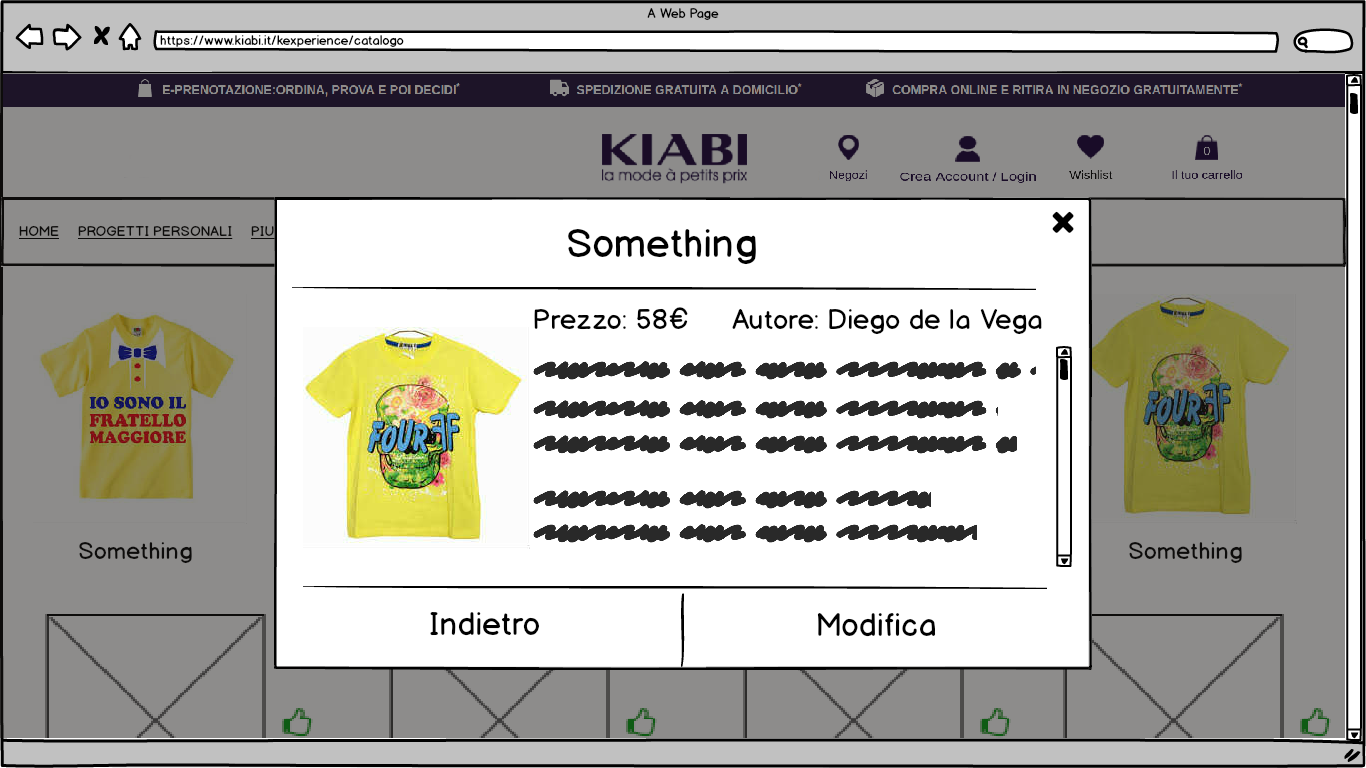
\includegraphics[width=0.9\textwidth]{../balsamiq/balsamiq_finale/Catalogodetails.png}
\caption{Catalogo - dettaglio}
\label{cat-dett}
\end{figure}

A fianco ad ogni immagine sono presenti tre bottoni che permettono agli
utenti loggati di votare positivamente o negativamente una maglietta e condividerla sui social (facebook, instagram e pinterest).
Nel caso un utente non loggato tentasse di votare, viene mostrato un
avviso che lo invita a fare il login o a registrarsi (Fig. \ref{cat-login}).

\begin{figure}[h]
\centering
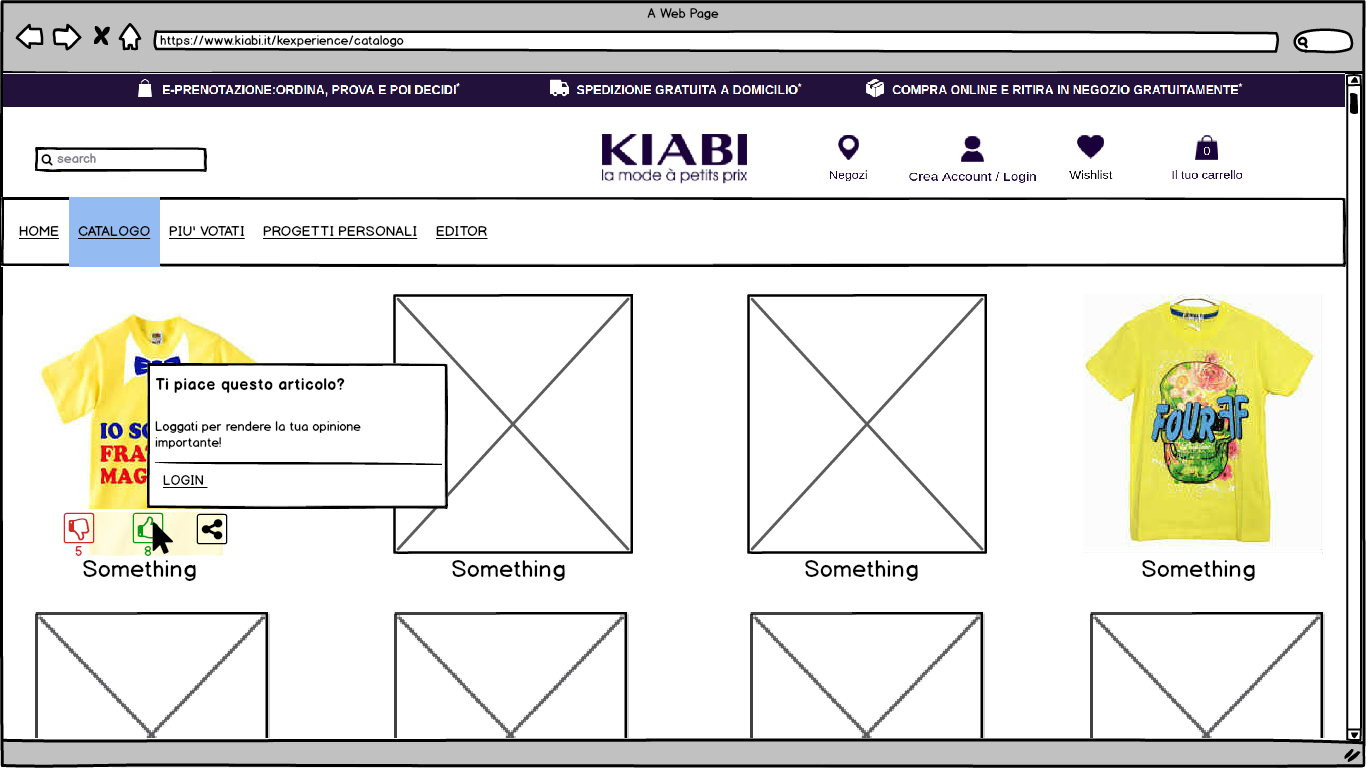
\includegraphics[width=0.9\textwidth]{../balsamiq/balsamiq_finale/Catalogologin.png}
\caption{Catalogo - login}
\label{cat-login}
\end{figure}

\newpage
\subsection{Più votati}\label{piuxf9-votati}

\begin{figure}[h]
\centering
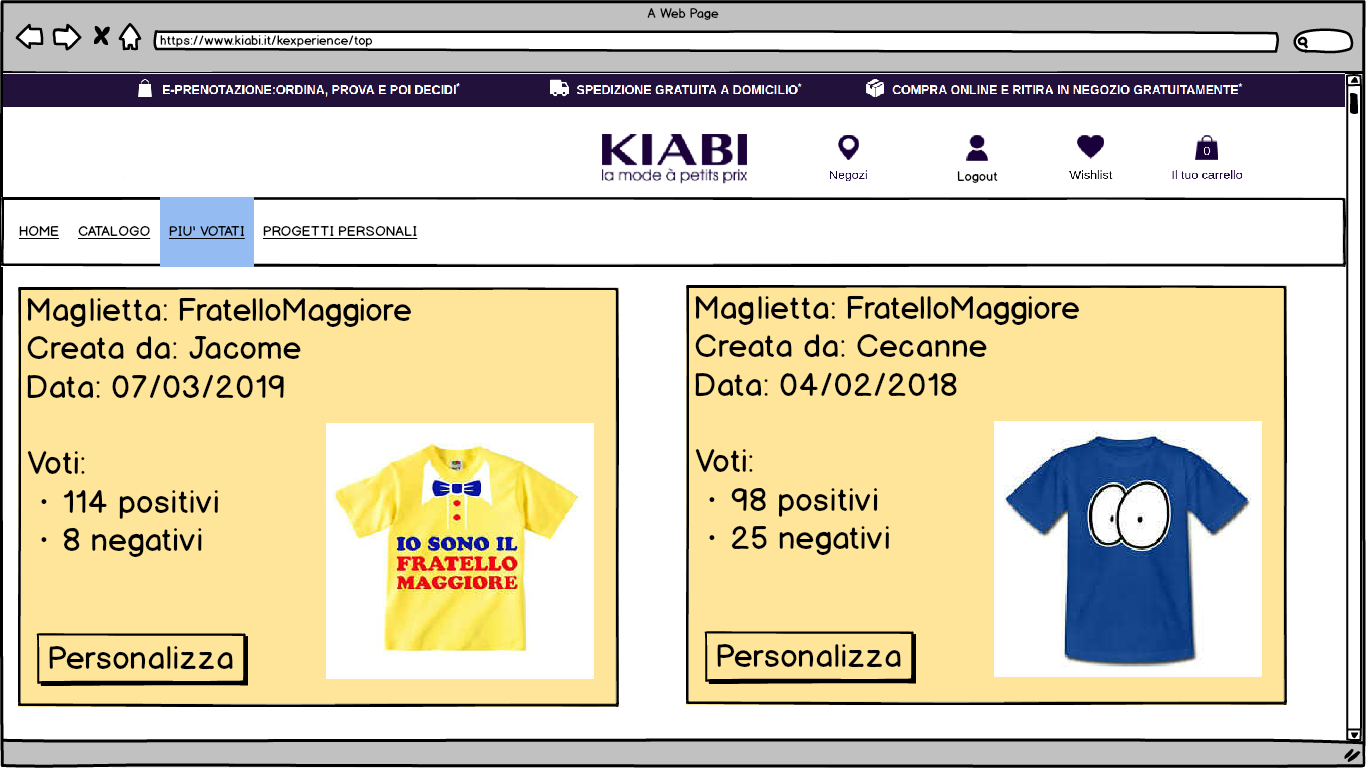
\includegraphics[width=0.9\textwidth]{../balsamiq/balsamiq_finale/MostRated.png}
\caption{Più votati}
\label{most-rated}
\end{figure}

In questa pagina sono mostrate, ordinate per numero di voti, le
magliette più votate dall'utenza (Fig. \ref{most-rated}). Per ogni maglietta sono mostrati
il nome dell'autore, il numero di voti, la data di creazione ed il titolo del
progetto. Premendo sul bottone personalizza si può modificare la
maglietta e procedere con l'acquisto oppure salvarla nei propri progetti personali.

\newpage
\hypertarget{progetti-personali}{%
\subsection{Progetti personali}\label{progetti-personali}}

\begin{figure}[h]
\centering
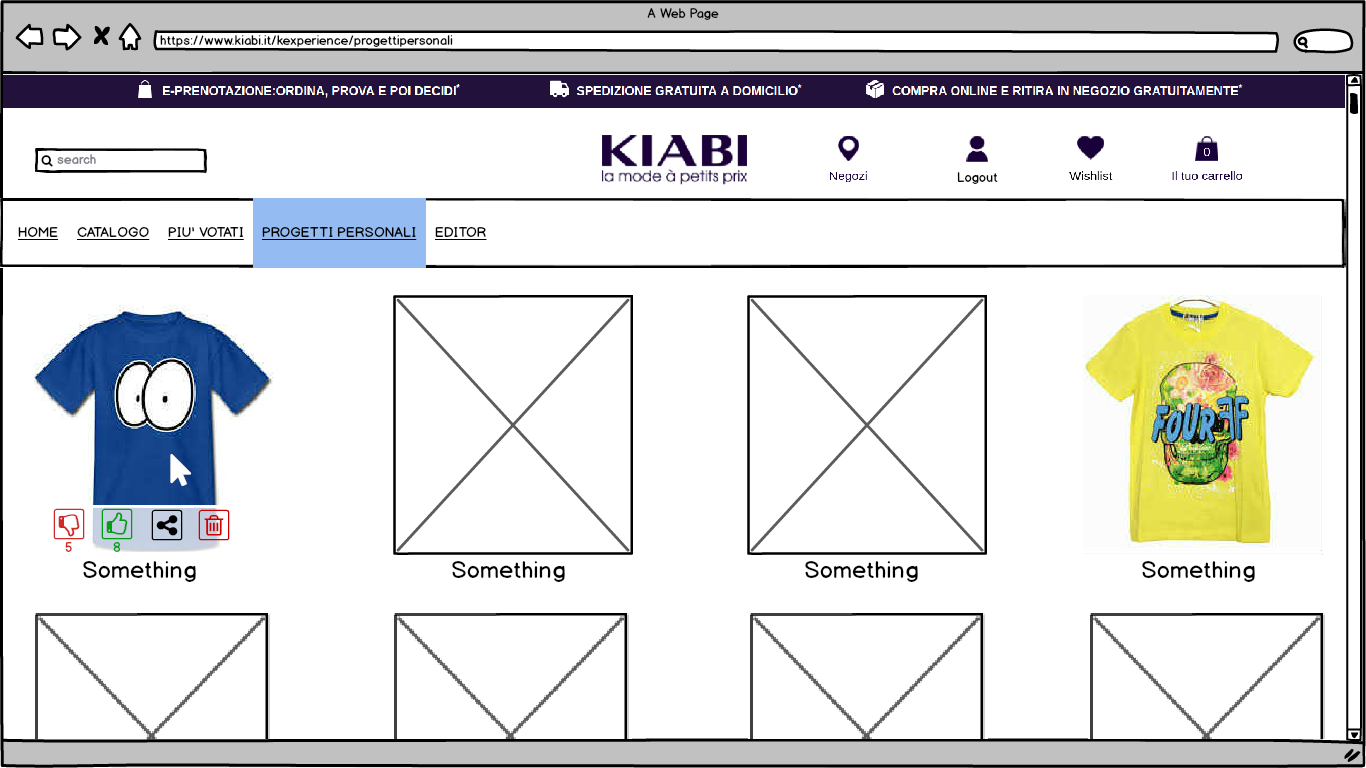
\includegraphics[width=0.9\textwidth]{../balsamiq/balsamiq_finale/ProgettiPersonali.png}
\caption{Progetti personali}
\label{prog-pers}
\end{figure}

In questa sezione (Fig \ref{prog-pers}) vengono elencati i progetti salvati dall'utente. Per ogni progetto, sull'hover del mouse, vengono mostrate le opzioni di condivisione sui social, visione dei "like" e "dislike" ricevuti ed eliminazione. Invece premendo sul progetto si apre un modale riepilogativo (Fig. \ref{prog-pers-dett}), da cui è possibile procedere alla personalizzazione.

\begin{figure}[h]
\centering
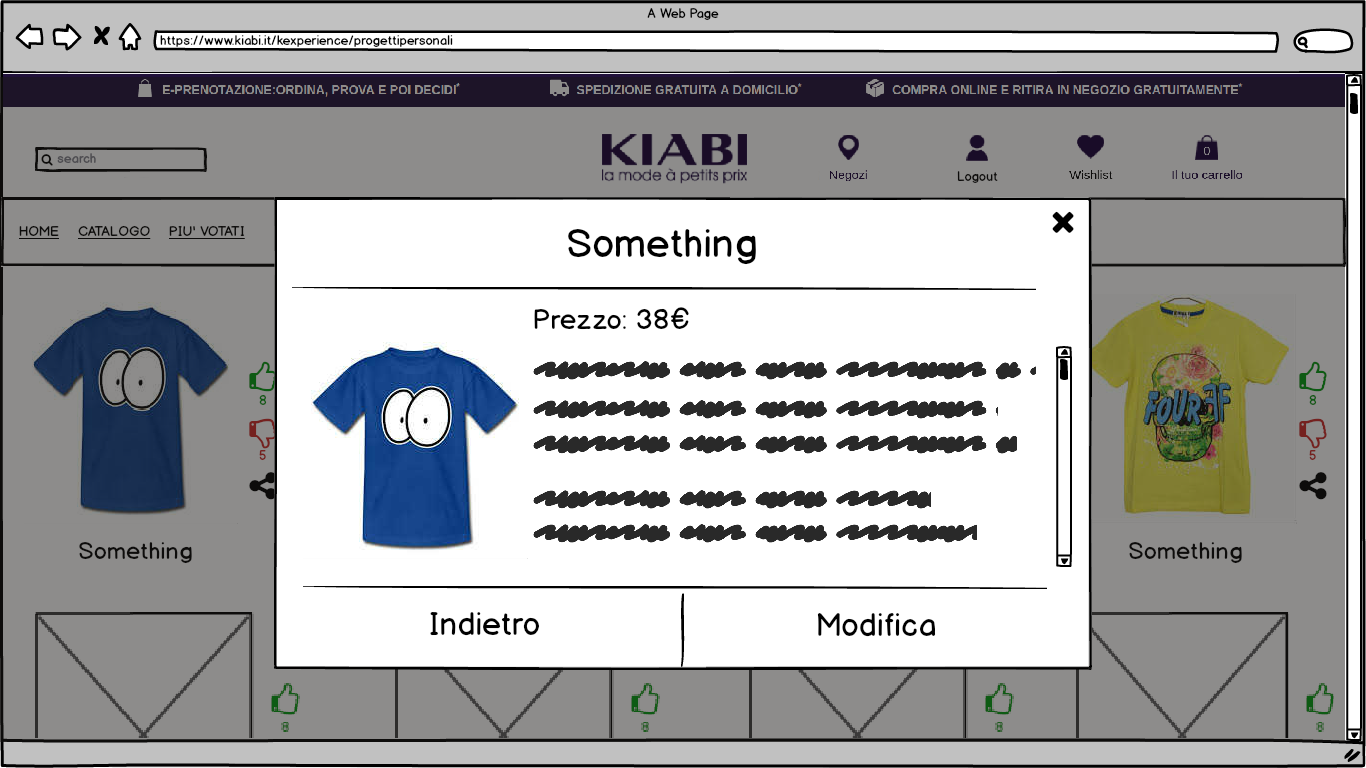
\includegraphics[width=0.9\textwidth]{../balsamiq/balsamiq_finale/ProgettiPersonalidetails.png}
\caption{Progetti personali - dettagli}
\label{prog-pers-dett}
\end{figure}

\newpage
\hypertarget{valutazione-della-progettazione}{%
\chapter{Valutazione della
progettazione}\label{valutazione-della-progettazione}}

Per coerenza con l'ispezione dei sistemi esistenti si è utilizzata un'analisi basata sulle dieci euristiche di Nielsen e Molich con l'aggiunta di tre euristiche di Weinshenk e Barker.

L'analisi è stata ripetuta perfezionando il sistema fino al raggiungimento di un risultato soddisfacente per i membri del team di sviluppo.

\section{Ispezione}\label{ispezione}

\subsection{Analisi diretta}

La pagina iniziale di Kids Experience mostra in modo chiaro ed evidente lo scopo del sito: creare una maglietta personalizzata. 

Gli elementi che caratterizzano questa pagina sono il bottone "Crea!" e il nostro slogan "La creatività è quel processo che dà vita a un nuovo prodotto."

Per quanto riguarda la navigazione, il sito è diviso in quattro macroaree per l'utente non loggato, mentre l'utente loggato può visitare un'ulteriore macroarea. 

\newpage
\begin{longtable}[]{@{}lll@{}}
\toprule
& Utente loggato & Utente non loggato\tabularnewline
\midrule
\endhead
Homepage & X & X\tabularnewline
Editor & X & X\tabularnewline
Progetti personali & X &\tabularnewline
Catalogo & X & X\tabularnewline
Più votati & X & X\tabularnewline
\bottomrule
\end{longtable}

Le differenze tra i due tipi di utente sono il poter votare o meno un prodotto nel catalogo, la possibilità di portare a termine un acquisto e salvare un proprio progetto.

A livello di layout e visual design, il prodotto mantiene un insieme di colori, icone ed elementi consistente ed offre in ogni pagina solo le informazioni essenziali. Laddove non è chiara la relazione tra elementi, sono presenti degli hint.

Kiabi offre già una sezione FAQ per utenti più esperti, che abbiamo ampliato con le domande maggiormente fatte in fase di test e un servizio di chat con un operatore per i nuovi arrivati.

\subsection{Analisi inversa} 

Euristiche non rispettate:

\begin{itemize}
\item \textbf{Controllo e libertà}: l'utente non ha modo di entrare direttamente nell'editor senza passare prima da un'altra pagina del sito;

\item \textbf{Flessibilità ed efficienza d'uso}: il sistema non offre delle shortcut per gli utenti più esperti;

\item \textbf{Riconoscimento anzichè ricordo}: le modifiche apportate alla maglietta sono visibili live solamente nel modello posto all'interno dell'editor. Non è possibile avere una lista completa, corredata di prezziario, delle modifiche apportate;

\item \textbf{Aiuto all'utente}: alcuni errori dovuti da azioni possibili solo per l'utente loggato, non erano ben specificate;
\end{itemize}

Le modifiche proposte alla fine dell'ispezione sono:
\begin{itemize}
\item Inserimento della voce "Editor" all'interno della navabar di Kids Experience;
\item Inserimento nell'editor di una "Lista delle modifiche" in cui sono presenti tutte le modifiche apportate, il loro costo unitario e la possibilità di eliminazione;
\item Inserimento di piccoli modali informativi prima di far eseguire azioni che richiedono all'utente il login o la registrazione; 
\end{itemize}



\hypertarget{test-utente}{%
\section{Test utente}\label{test-utente}}

Vista la mancanza di un team specializzato per il testing del software,
si è deciso di utilizzare il Discount Usability Testing. Questa
tipologia di testing risulta essere più formale, intuitiva, sequenziale
e a buon mercato, ma comunque utile come test formativo.

\hypertarget{protocollo-di-testing-1}{%
\subsection{Protocollo di testing}\label{protocollo-di-testing-1}}

Si è scelto di svolgere quattro test, con sei utenti diversi, per
mantenere la consistenza con i test precedenti. I test, secondo la
metodologia discout usability testing, sono stati eseguiti in maniera
sequenziale, migliorando il design dopo ogni iterazione.

I test sono eseguiti con il protocollo definito nel capitolo \ref{protocollo-di-testing}, usando i wireframe mostrati nel capitolo \ref{wireframes}.

\hypertarget{task-considerati}{%
\subsection{Task considerati}\label{task-considerati}}

I task considerati per gli utenti sono:

\begin{enumerate}
\def\labelenumi{\arabic{enumi}.}
\tightlist
\item
  Acquistare una maglietta personalizzata
\item
  Votare una maglietta personalizzata tra quelle presenti nel catalogo
\item
  Modificare un progetto tra quelli \emph{più votati}
\item
  Creare una maglietta personalizzata e salvarla
\end{enumerate}

Gli utenti scelti sono:

\begin{itemize}
\tightlist
\item
  Marco, 23 anni, ha una conoscenza del computer nella media e  ha due sorelle minori che adorano la cultura orientale.
\item
  Viviana, 24 anni, ha una discreta conoscenza del computer, sognatrice,
  sportiva, ha una nipote a cui piacciono le serie TV.
\item
  Antonio, 28 anni, ha una buona conoscenza del web, in particolare i
  social. È un influencer (549k followers) e frequenta un master in
  psicologia.
\item
  Lorenzo, 36 anni, livello tecnologico medio, ma con ottima conoscenza
  del mondo della moda.
\item
  Alessandro, 25 anni, conoscenza media del computer, ha un fratello
  minore. Studia lettere moderne e adora leggere fumetti.
\item
  Giorgia, 29 anni, laureata in ingegneria informatica, guarda solo i
  film d'azione e nel tempo libero adora fa da babysitter ai cuginetti,
  che adora.
\end{itemize}

Sono state scelte le seguenti metriche per la valutazione dell'usabilità
del sistema:

\begin{itemize}
\tightlist
\item
  Svolgimento: successo, fallimento
\item
  Errori: Nielsen
\item
  Efficienza: alta, media, bassa
\end{itemize}

\hypertarget{raccolta-dati}{%
\subsubsection{Raccolta dati}\label{raccolta-dati}}

\begin{longtable}[]{@{}lllll@{}}
\toprule
Marco & Task 1 & Task 2 & Task 3 & Task 4\tabularnewline
\midrule
\endhead
Svolgimento & Successo & Fallimento & Successo & Successo\tabularnewline
Errori & Errore grave & Errore catastrofico & / & Errore
cosmetico\tabularnewline
Efficienza & Media & Alta & Alta & Alta\tabularnewline
\bottomrule
\end{longtable}

Risposte questionario SUS:

\begin{longtable}[]{@{}ll@{}}
\toprule
Domanda & Risposta\tabularnewline
\midrule
\endhead
1 & 3\tabularnewline
2 & 2\tabularnewline
3 & 4\tabularnewline
4 & 1\tabularnewline
5 & 3\tabularnewline
6 & 2\tabularnewline
7 & 4\tabularnewline
8 & 2\tabularnewline
9 & 5\tabularnewline
10 & 2\tabularnewline
\bottomrule
\end{longtable}

\begin{longtable}[]{@{}lllll@{}}
\toprule
Viviana & Task 1 & Task 2 & Task 3 & Task 4\tabularnewline
\midrule
\endhead
Svolgimento & Successo & Successo & Successo & Successo\tabularnewline
Errori & Errore minore & / & / & /\tabularnewline
Efficienza & Media & Alta & Alta & Alta\tabularnewline
\bottomrule
\end{longtable}

Risposte questionario SUS:

\begin{longtable}[]{@{}ll@{}}
\toprule
Domanda & Risposta\tabularnewline
\midrule
\endhead
1 & 3\tabularnewline
2 & 2\tabularnewline
3 & 2\tabularnewline
4 & 1\tabularnewline
5 & 3\tabularnewline
6 & 2\tabularnewline
7 & 4\tabularnewline
8 & 1\tabularnewline
9 & 4\tabularnewline
10 & 1\tabularnewline
\bottomrule
\end{longtable}

\begin{longtable}[]{@{}lllll@{}}
\toprule
Antonio & Task 1 & Task 2 & Task 3 & Task 4\tabularnewline
\midrule
\endhead
Svolgimento & Successo & Successo & Successo & Successo\tabularnewline
Errori & / & / & / & /\tabularnewline
Efficienza & Alta & Alta & Alta & Alta\tabularnewline
\bottomrule
\end{longtable}

Risposte questionario SUS:

\begin{longtable}[]{@{}ll@{}}
\toprule
Domanda & Risposta\tabularnewline
\midrule
\endhead
1 & 5\tabularnewline
2 & 2\tabularnewline
3 & 5\tabularnewline
4 & 1\tabularnewline
5 & 4\tabularnewline
6 & 1\tabularnewline
7 & 3\tabularnewline
8 & 1\tabularnewline
9 & 4\tabularnewline
10 & 1\tabularnewline
\bottomrule
\end{longtable}

\begin{longtable}[]{@{}lllll@{}}
\toprule
Lorenzo & Task 1 & Task 2 & Task 3 & Task 4\tabularnewline
\midrule
\endhead
Svolgimento & Successo & Successo & Successo & Successo\tabularnewline
Errori & Errore minore & / & / & /\tabularnewline
Efficienza & Media & Alta & Alta & Alta\tabularnewline
\bottomrule
\end{longtable}

Risposte questionario SUS:

\begin{longtable}[]{@{}ll@{}}
\toprule
Domanda & Risposta\tabularnewline
\midrule
\endhead
1 & 4\tabularnewline
2 & 4\tabularnewline
3 & 5\tabularnewline
4 & 2\tabularnewline
5 & 3\tabularnewline
6 & 3\tabularnewline
7 & 4\tabularnewline
8 & 2\tabularnewline
9 & 3\tabularnewline
10 & 1\tabularnewline
\bottomrule
\end{longtable}

\begin{longtable}[]{@{}lllll@{}}
\toprule
Alessandro & Task 1 & Task 2 & Task 3 & Task 4\tabularnewline
\midrule
\endhead
Svolgimento & Successo & Successo & Successo & Successo\tabularnewline
Errori & Errore grave, cosmetico & Errore minore & / & /\tabularnewline
Efficienza & Bassa & Media & Alta & Alta\tabularnewline
\bottomrule
\end{longtable}

\begin{longtable}[]{@{}ll@{}}
\toprule
Domanda & Risposta\tabularnewline
\midrule
\endhead
1 & 4\tabularnewline
2 & 3\tabularnewline
3 & 4\tabularnewline
4 & 1\tabularnewline
5 & 5\tabularnewline
6 & 2\tabularnewline
7 & 4\tabularnewline
8 & 2\tabularnewline
9 & 4\tabularnewline
10 & 1\tabularnewline
\bottomrule
\end{longtable}

\begin{longtable}[]{@{}lllll@{}}
\toprule
Giorgia & Task 1 & Task 2 & Task 3 & Task 4\tabularnewline
\midrule
\endhead
Svolgimento & Successo & Successo & Successo & Successo\tabularnewline
Errori & Errore cosmetico & / & / & /\tabularnewline
Efficienza & Alta & Alta & Alta & Alta\tabularnewline
\bottomrule
\end{longtable}

\begin{longtable}[]{@{}ll@{}}
\toprule
Domanda & Risposta\tabularnewline
\midrule
\endhead
1 & 4\tabularnewline
2 & 1\tabularnewline
3 & 5\tabularnewline
4 & 1\tabularnewline
5 & 4\tabularnewline
6 & 2\tabularnewline
7 & 4\tabularnewline
8 & 1\tabularnewline
9 & 5\tabularnewline
10 & 1\tabularnewline
\bottomrule
\end{longtable}

\hypertarget{punteggi-questionario-sus}{%
\subsubsection{Punteggi questionario
SUS}\label{punteggi-questionario-sus}}

Al termine di ogni test è stato proposto ad ogni utente un questionario
di soddisfazione composto da dieci affermazioni. Le risposte sono state
date utilizzando la \emph{Scala di Likert} con valori compresi tra 1 e
5, dove 1 significa essere completamente in disaccordo con
l'affermazione data, mentre 5 essere completamente d'accordo. Il
risultato ottenuto, compreso in una scala che va da 0 a 100, è
nettamente più alto rispetto a quello ottenuto dai sitemi esistenti.

\begin{longtable}[]{@{}lllllllllllll@{}}
\caption{Riepilogo risposte SUS}\tabularnewline
\toprule
& 1 & 2 & 3 & 4 & 5 & 6 & 7 & 8 & 9 & 10 & Somma & Totale\tabularnewline
\midrule
\endfirsthead
\toprule
& 1 & 2 & 3 & 4 & 5 & 6 & 7 & 8 & 9 & 10 & Somma & Totale\tabularnewline
\midrule
\endhead
Marco & 3 & 2 & 4 & 1 & 3 & 2 & 4 & 2 & 5 & 2 & 30 & 75\tabularnewline
Viviana & 3 & 2 & 2 & 1 & 3 & 2 & 4 & 1 & 4 & 1 & 29 &
72,5\tabularnewline
Antonio & 5 & 2 & 5 & 1 & 4 & 1 & 3 & 1 & 4 & 1 & 35 &
87,5\tabularnewline
Lorenzo & 4 & 4 & 5 & 2 & 3 & 3 & 4 & 2 & 3 & 1 & 27 &
67,5\tabularnewline
Alessandro & 4 & 3 & 4 & 1 & 5 & 2 & 4 & 2 & 4 & 1 & 32 &
80\tabularnewline
Giorgia & 4 & 1 & 5 & 1 & 4 & 2 & 4 & 1 & 5 & 1 & 36 & 90\tabularnewline
\bottomrule
\end{longtable}

Nell'elenco di seguito vengono evidenziati gli errori commessi dagli
utenti nell'utilizzo di Kids Experience. Ad ogni errore verrà attribuito
un codice per identificarlo nei grafici seguenti.

\begin{itemize}
\item I link bambino e bambina presenti nella navbar della homepage di Kiabi venivano spesso scelti come link di accesso a Kids Experience (\textbf{E1})
\item Spesso gli utenti premevano il bottone per il salvataggio di una maglietta invece che acquistarla nel task 1 (\textbf{E2})
\item Il tasto indietro nella scheda di personalizzazione non sempre veniva riconosciuto (\textbf{E3})
\item Il tasto chiudi 'X' nella scheda di personalizzazione non sempre veniva vista (\textbf{E4})
\item Alcuni utenti hanno evidenziato una ridondanza nei path per le personalizzazioni dell'editor (\textbf{E5})
\item Alcuni utenti hanno notato delle inconsistenze nella lingua di alcuni link (\textbf{E6})
\item Non tutti hanno avuto subito chiaro che le modifiche fossero mostrate in tempo reale (\textbf{E7})
\end{itemize}

La seguente tabella classifica gli errori riscontrati in base
all'impatto, utilizzando la classificazione proposta da Nielsen.

\begin{longtable}[]{@{}llllll@{}}
\toprule
Errore & Implementativo & Catastrofico & Grave & Minore &
Cosmetico\tabularnewline
\midrule
\endhead
E1 & & & X & &\tabularnewline
E2 & & X & & &\tabularnewline
E3 & & & & X & X\tabularnewline
E4 & & & & X & X\tabularnewline
E5 & & & & & X\tabularnewline
E6 & & & & & X\tabularnewline
E7 & & & X & &\tabularnewline
\bottomrule
\end{longtable}

\hypertarget{curve-durgenza}{%
\subsubsection{Curve d'urgenza}\label{curve-durgenza}}

La curva d'urgenza è un grafico bidimensionale ``impatto vs frequenza''
in cui sono presenti i vari errori riscontrati.

\begin{figure}[h]
\centering
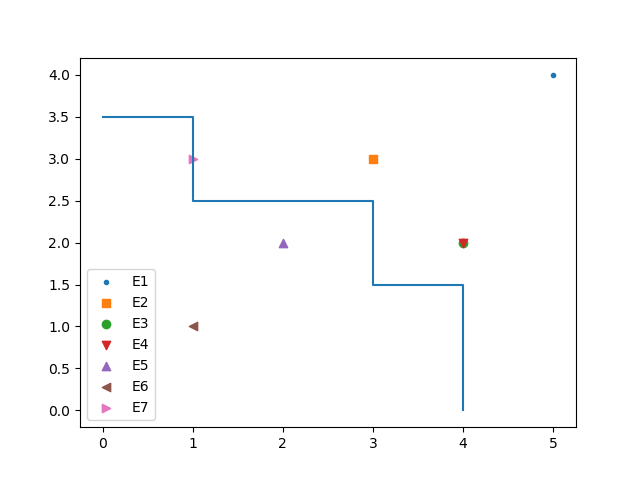
\includegraphics{img/curva_urgenza.png}
\caption{Curve d'urgenza}
\end{figure}

\hypertarget{conclusione}{%
\chapter{Conclusione}\label{conclusione}}

Kids Experience nasce con l'intento di rilanciare l'attività nel settore dell'abbigliamento per bambini di Kiabi. 
È un'idea innovativa in quanto i negozi della grande distribuzione non sono soliti a creare prodotti personalizzati in base ai gusti dell'utente. 

Il sistema è stato creato da zero, prendendo come riferimento il sito Kiabi.it. 
I test utente effettuati sul sistema esistente hanno permesso di individuare gli errori più comuni, permettendoci di non ripeterli nella realizzazione di Kids Experience.
I successivi test effettuati in modo iterativo su Kids Experience hanno consentito di correggere di volta in volta gli errori ritenuti più gravi.

Visti i risultati ottenuti nei questionari SUS possiamo affermare con certezza che Kids Experience ha un'alta \emph{Learnability}, ovvero un'alta facilità di apprendimento, ed una \emph{Usability} media. Questi risultati sono particolarmente soddisfacenti se consideriamo che il prodotto offerto è una novità per questo tipo di aziende e propone un concetto nuovo come l'estrema personalizzazione di magliette.

Per quanto riguarda gli sviluppi futuri, si prevede un buon margine di miglioramento andando sia ad ampliare le categorie di prodotti personalizzabili sia aumentando il numero di personalizzazioni disponibili.

\newpage
\section{Licenza}\label{licenza}


\includegraphics{img/licenza.png}

Quest'opera è rilasciata sotto una licenza
\href{https://creativecommons.org/licenses/by-nc-sa/4.0/}{Creative
Commons Attribution-NonCommercial-ShareAlike 4.0 International License}.

\bibliography{Relazione}
\bibliographystyle{unsrt}
\end{document}
